% !TeX spellcheck = cs_CZ
%---------------------------------------------------------------------------------------------------
% file SMPS.tex
%---------------------------------------------------------------------------------------------------
%========= Kapitola: Impulzně regulované napájecí zdroje ===========================================
\setchaptertoc
\chapter{Impulzně regulované napájecí zdroje}

  \section{Úvod}\label{aes:sec010}
    Spínané napájecí zdroje plní funkci stejnou jako zdroje se spojitou regulací. Vý\-ko\-no\-vý
    člen spínacích zdrojů je však zatěžován impulzně, tj. střídavě spínán a rozepínán. Lze tedy
    využít výhody impulzního režimu, tj. odebírat impulzní výkon podstatně větší, než je trvalý
    výkon při lineárním režimu regulátoru s týmž výkonovým členem. Spínací zdroje mají obecně větší
    účinnost než zdroje se spojitou regulací. Jsou výhodné zvláště tam, kde je velký rozdíl napětí
    na vstupu a výstupu regulátoru a kde jsou požadované malé rozměry. Impulzní regulace zajistí
    stabilizované výstupní napětí i pro velké změny vstupního napětí; účinnost zdroje se při tom
    téměř nemění. I přes větší obvodovou složitost jsou ekonomicky výhodnější, neboť jejich použití
    vede k podstatné energetické úspoře.
  
    Impulzně regulované zdroje však mají v porovnání se zdroji s lineární regulací i některé
    nevýhodné vlastnosti, například pomalejší reakci výstupního napětí na rychlé změny zatěžovacího
    výstupního proudu. Při požadavku malého zvlnění výstupního napětí se nesmí zanedbat vliv
    impulzního charakteru těchto zdrojů. Impulzně regulované zdroje jsou také zdrojem rušivých
    signálů, které jsou generovány spínacími prvky \cite[s.~112]{Hammembauer}.
       
  \section{Impulzní regulace ve výkonové elektronice}\label{aes:sec005}
    Základním principem a současně odlišností impulzní regulace od regulace klasické je v její
    \emph{nespojitosti}. To znamená, že nehledě na detailní realizaci, je výstupní napětí 
    stabilizováno zásahy regulačního členu pouze v určitých, časově omezených intervalech. Podstata 
    regulačního členu (regulátoru) tedy spočívá v řízení vzájemných časových relací aktivního a 
    pasivního intervalu pracovního cyklu v závislosti na velikosti zesílené regulační odchylky.
    
    Akční člen je tedy řízen dvouhodnotovým signálem, mající význam \emph{zapnutí} nebo 
    \emph{vypnutí} výkonové součástky. Následující příklad demonstruje, jak lze tento signál 
    vytvořit pomocí \textbf{pulzně-šířkové modulace} v simulátoru \ltLtspiceSW. V simulacích 
    některých topologií spínaných zdrojů bude místo zdroje s lineárně narůstajícím výstupním 
    napětím viz obr. \ref{enz:fig_pwm_wave} použita regulační odchylka.
    
    \begin{figure}[ht!]
      \centering
      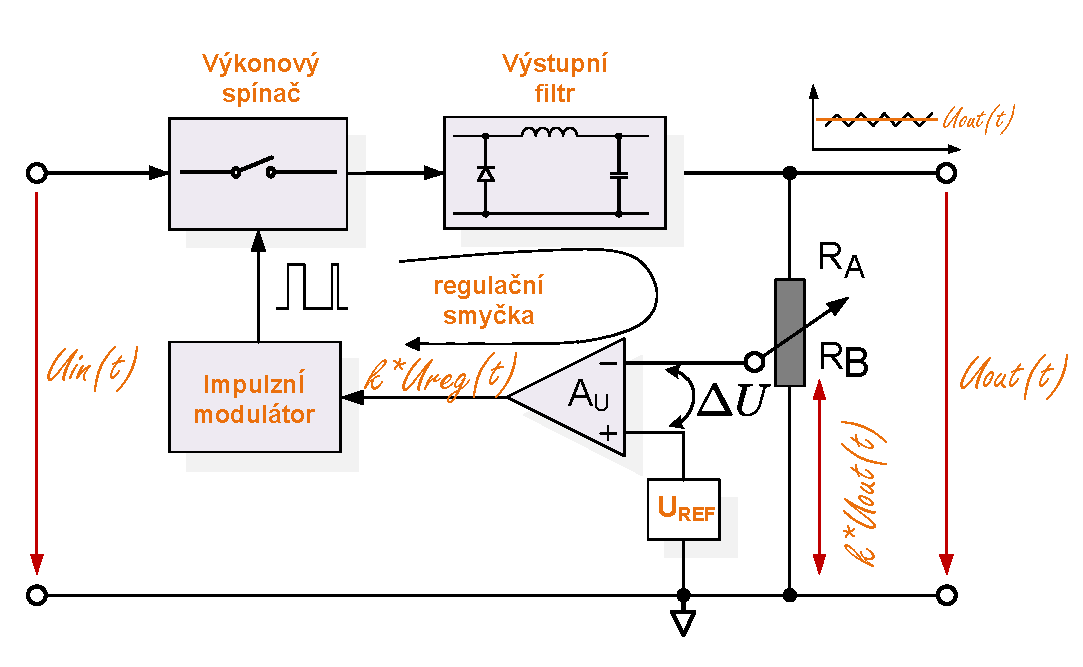
\includegraphics[width=0.8\linewidth]{hamm_schema_imp_reg.pdf}
      \caption[Schéma impulzního regulátoru]{Základní schéma impulzního regulátoru}
      \label{enz:fig_imp_reg_basic}
    \end{figure}
    
    Srovnáme-li pro názornost klasický a impulzní regulátor na úrovni blokových schémat, vidíme, že 
    obě jsou formálně dosti podobná. U obou nacházíme napěťový normál \texttt{Uref}, zesilovač 
    regulační odchylky \texttt{Au}, budící obvod i výkonový regulační člen a samozřejmě i 
    zpětnovazební smyčku. Tím však, snad až na základní podstatu regulační smyčky podobnost končí. 
    Funkčně jsou oba regulátory naprosto odlišné.
    
    U spojitého lineárního regulátoru ovládá odchylka výstupního napětí od jmenovité velikosti 
    spojitě okamžitý odpor výkonového regulačního členu v libovolném o\-kam\-ži\-ku tak, aby 
    výstupní napětí bylo konstantní. Z toho, jak je již známo, vyplývá velká poměrná výkonová 
    ztráta na regulačním členu a tedy i malá účinnost spojité regulace za běžných provozních 
    podmínek.
    
    Impulzní regulace obr. \ref{enz:fig_imp_reg_basic} umožňuje výrazně snížit výkonovou ztrátu na
    regulačním členu. V tomto případě pracuje regulační prvek (tranzistor) jako řízený spínač. 
    Proud jím tedy prochází pouze po určitý interval pracovního cyklu. Přitom okamžitá výkonová 
    ztráta v aktivním (sepnutém) stavu je vzhledem k $U_{CES}\rightarrow 0$ řádově menší, než u 
    lineárního regulátoru. Další předností je, že velikost ztráty v podstatě nezávisí na rozdílu 
    vstupního a výstupního napětí, ale prakticky pouze na kolektorovém proudu tranzistoru.
    
    Možnost použít spínací regulační člen při stabilizaci stejnosměrného napětí je podmíněna jeho 
    vzájemnou součinností s filtračním členem, který na rozdíl od aplikace ve spojitém regulátoru 
    musí mít výrazný akumulační charakter. Uspořádání filtru, který je pro větší výkony vždy typu 
    LC, je podřízeno topologii měniče. Princip činnosti nerozlučně vázané dvojice spínač - 
    akumulační výstupní filtr spočívá v akumulaci energie, která je v aktivním intervalu odebrána 
    ze zdroje, aby mohla být v následujícím pasivním intervalu (spínač vypnut) dodávána z filtru do 
    zátěže \cite[s.~121]{Hammembauer}.
           
    % --------example: PWM gen ------------------------
    % \label{AES:exam003}
    % !TeX spellcheck = cs_CZ
\begin{example}\label{AES:exam003}
  Na obr. \ref{enz:fig_pwm_gen} je realizován generátor šířkově modulovaného signálu pro
  simulátor \texttt{LTSpice}, jenž s výhodou využívá komponenty \texttt{B-source}, umožňující
  behaviorální popis požadovaného průběhu.

   {\centering
    \captionsetup{type=figure} 
    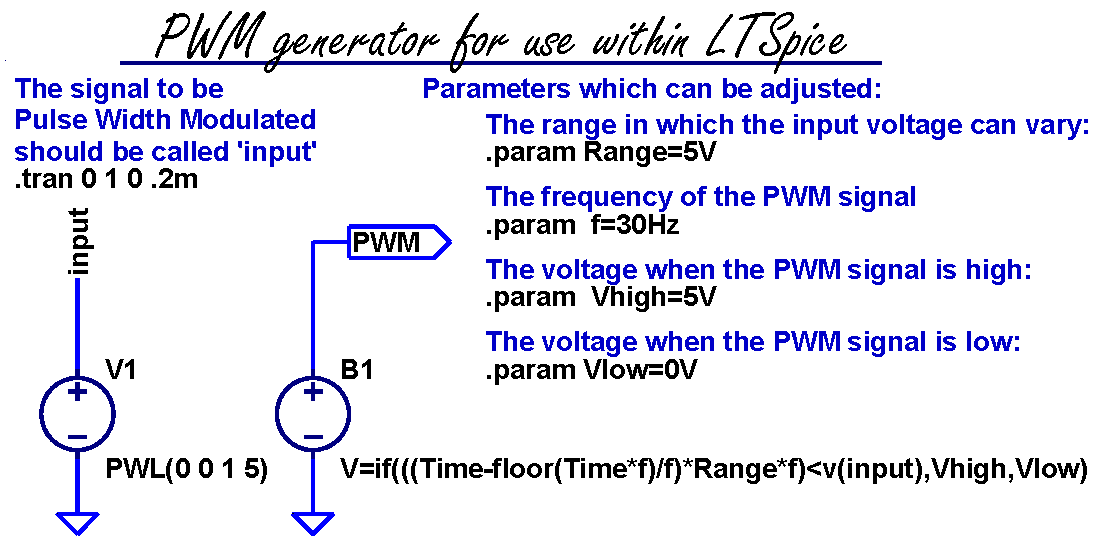
\includegraphics[width=0.8\linewidth]{LTspice_pwm_gen.pdf}
    \captionof{figure}{Realizace PWM generátoru pomocí komponenty B-source \emph{(Arbitrary 
               behavioral voltage or current source)} v LTSpice (soubor \texttt{pwm.asc})}
    \label{enz:fig_pwm_gen}
  \par}
  Podrobnějším pohledem na zápis rovnic dle obr. \ref{enz:fig_pwm_gen}, lze dojít k závěru, že
  zdroj \texttt{B1} na svůj výstup vnutí hodnotu parametru \texttt{Vhigh}, nebo \texttt{Vlow},
  podle výsledku rozhodovací funkce \texttt{if}. Tj. jeli \texttt{Time-floor(Time*f)/f)*Range*f)} 
  větší než \texttt{V(input)}, bude na výstupu $V_{high}= \SI{5}{\volt}$, v opačném případě 
  $V_{low} = 0V$. Funkce \texttt{floor} zaokrouhluje hodnotu svého argumentu na celé číslo 
  (\texttt{integer}), což vede na schodovitý průběh a funkce \texttt{Time} umožňuje do vztahu vnést 
  okamžitou hodnotu simulačního času. Vzájemný odečtením získáme pilový průběh, kterým se komparuje 
  s okamžitou hodnotou zdroje \texttt{V(input)}.

    {\centering
     \captionsetup{type=figure} 
     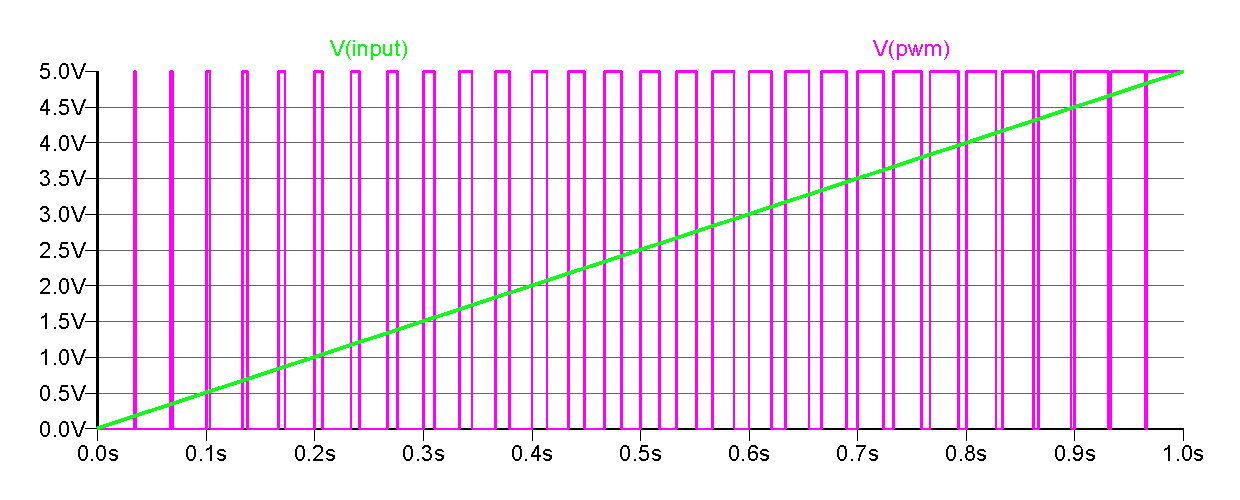
\includegraphics[width=1\linewidth]{LTspice_pwm_wave.pdf}
     \captionof{figure}{Výstupní signál \texttt{V(pwm)} z PWM generátoru na obr. 
                \ref{enz:fig_pwm_gen}  má-li rozhodovací napětí \texttt{V(in)} lineární charakter}
     \label{enz:fig_pwm_wave}
   \par}       
\end{example}   
    %--------------------------------------------------

    \subsection{Vymezení pojmů a základních požadavků}\label{aes:sec012}
      DC - DC měniče jsou obvody sloužící k regulaci elektrické energie, které mění vstupní
      stejnosměrné napětí \(U_1\) na jiné výstupní stejnosměrné napětí \(U_2\). Budeme se přitom 
      zabývat měniči tzv. \emph{napěťového typu}, což jsou měniče napájené konstantním vstupním 
      napětím z napěťového zdroje, nikoliv proudem, z proudového zdroje. V této kapitole se omezíme 
      pouze na měniče bez transformátoru, které tedy neumožňuji galvanické oddělení výstupu od 
      vstupu \cite{Patocka}.
      
      \begin{figure}[ht!]
        \centering
        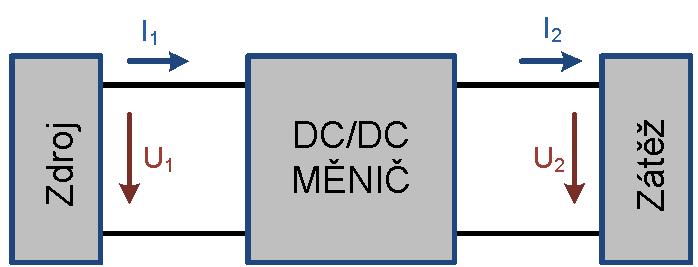
\includegraphics[width=0.5\linewidth]{patocka_pracovni_kvadranty_sch.pdf}
        \caption{Označení vstupních a výstupních veličin DC/DC měniče.}
        \label{enz:fig_005}
      \end{figure}
      
      Každý měnič sestává z vlastního silového obvodu a řídicí elektroniky (regulačních obvodů).
      Silové obvody nesmí využívat při regulaci energie rezistorů a proto se mohou skládat jen ze
      \textbf{spínačů} a \textbf{akumulačních prvků}, tj. \emph{indukčnosti} a \emph{kapacit}.
      
      DC/DC měniče mohou přenášet energii z principu oběma směry. Mohou tedy čerpat energii ze
      zdroje a dodávat ji do zátěže nebo také opačně energii čerpat ze zátěže a dodávat ji do
      zdroje. Pojmy zátěž a zdroj je proto nutné chápat v širším slova smyslu.
      
      \begin{figure}[ht!]
        \centering
        \subcaptionbox{     \label{enz:fig_nahr_sch_aku}}{\luafigure[0.4]{patocka_aktivni_zatez_nahrad_sch.pdf}}
        \hspace{1cm}
        \subcaptionbox{\label{enz:fig_nahr_sch_ss_motor}}{\luafigure[0.4]{patocka_aktivni_zatez_ss_mot_nahrad_sch.pdf}}
        \caption{Aktivní zátěž: a) náhradní schéma akumulátoru; b) náhradní schéma stejnosměrného 
          elektromotoru s cizím buzením}
        \label{enz:fig_aktivni_zatez}
      \end{figure}        
      \begin{itemize}[noitemsep]
        \item Zdrojem s konstantním napětím $U_1$, schopným dodávat i akumulovat energii, je
              \textbf{akumulátor}. Použijeme-li jako zdroj např.\emph{ usměrňovač se sběrným 
              kondenzátorem}, pak není schopen dlouhodobě jímat energii z měniče, tj. dlouhodobě 
              nesmí ve střední hodnotě převládat směr proudu do kladné svorky zdroje (krátkodobě, 
              v okamžité hodnotě, je takový směr možný). Nabíjením sběrného kondenzátoru by totiž 
              rostlo napětí $U_1$. Tomu lze zabránit přeměnou dodávané energie na teplo ve 
              vybíjecím rezistoru, či na Zenerově diodě, zapojené paralelně ke sběrnému 
              kondenzátoru.
        \item Z hlediska schopnosti \emph{spotřeby} či \emph{dodávky} energie, lze rozlišovat 
              zátěž \emph{aktivní} a \emph{pasivní}. Aktivní zátěži je opět např. akumulátor, ale 
              třeba i stejnosměrný motor. Jeho náhradní zapojení, platné v ustáleném stavu, je 
              uvedeno na obr. \ref{enz:fig_nahr_sch_ss_motor}. Vnitřní rotační (pohybové) 
              indukované napětí je úměrně otáčkám, proud pak momentu na hřídeli a to včetně 
              znamének.
      \end{itemize}
      

      Teče-li proud ve  střední hodnotě do zátěže (\(+I\)), pak motor pohání, tj. mění elektrickou
      energii na mechanickou (pracuje v \emph{motorickém režimu}). Teče-li ze zátěže (\(-I\)), pak
      motor brzdí, tj. mění z vnějšku dodávanou mechanickou energii na energii elektrickou
      (pracuje v \emph{generátorickém režimu}).       
      
      Označme si vstupní a výstupní napětí a proud měniče podle obr. \ref{enz:fig_005}. Podle 
      polarity výstupního napětí $U_2$ a výstupního proudu $I_2$ může měnič pracovat ve čtyřech 
      kvadrantech tzv.\textbf{ VA-roviny} (viz obr. \ref{aes:fig072}).

      \luagraphic[0.8]{aes_fig072.pdf}{Pracovní kvadranty ve VA rovině.}{aes:fig072}

      V kvadrantech \emph{1} i \emph{3} dodává měnič energii do zátěže. Je-li zátěží motor, tak
      pohání. Pasivní zátěže mohou pracovat pouze v těchto kvadrantech. V kvadrantech \emph{2} a
      \emph{4} dodává aktivní zátěž energii zpět do měniče. Jde-li o motor\footnote{Velikost
      napětí ss. motoru je úměrná otáčkám (rychlosti), polarita je dána směrem otáčení
      (uvažujeme motor s cizím buzením, např. s permanentními magnety). Velikost proudu je
      úměrná momentu na hřídeli, polarita je opět dána směrem momentu, tj. zda motor brzdí či
      pohání. Je třeba si povšimnout, že přechod mezi generátorickým a motorickým režimem mezi
      kvadranty 2 a 1 nebo mezi 3 a 4 (tj. takový, kdy se nemění polarita napětí, ale jen
      proudu) vůbec nemusí být na hřídeli motoru opticky pozorovatelný, neboť v dané chvíli
      přechodu se změní jen znaménko momentu (proudu) a přesto otáčky hřídele mohou být
      konstantní.}, pak brzdí.
      
      \textbf{Pravidla pro konstrukci silového obvodu}:
      \begin{enumerate}[noitemsep]
        \item \textbf{Indukčnost} nesmí být zapojena paralelně ke vstupu či výstupu ( napětí zde 
              nemá nulovou střední hodnotou).
        \item \textbf{Kapacita} nesmí být zapojena do série se vstupní nebo výstupní svorkou 
              měniče (proud zde nemá nulovou střední hodnotou).
        \item Jako akumulační prvek nelze použít samostatně kapacitu, není-li v obvodu použita
              ještě indukčnost (protože by v měniči napěťového typu docházelo k nepřípustnému
              nárazovému nabíjení kondenzátoru zkratovým proudem). Čili měnič napěťového typu
              musí obsahovat alespoň jednu indukčnost.
        \item Žádný \textbf{spínač} nesmí zkratovat vstup ani výstup měniče.
      \end{enumerate}
      
      \subsubsection{Nejjednodušší měniče s jediným akumulačním 
        prvkem}\label{ENZ:tit_menice_s_1_aku_prvkem} 
        Pro výchozí představu, vysvětlující princip činnosti, vytvoříme silový obvod měniče ze
        dvou prvků. Bude to indukčnost  \emph{L} a ideální přepínač. Vezmeme-li v úvahu výše 
        uvedená omezení, existují podle obr. \ref{enz:fig_002} jen tři způsoby, jak takový měnič 
        zapojit \cite{Patocka}.
      
        \begin{figure}[ht!]  %\ref{enz:fig_002}
          \centering
          \subcaptionbox{\(U_x < U_1\) \label{enz:fig_stepdown}}         
            {\luafigure[0.35]{patocka_step_down_princip.pdf}}     
          \subcaptionbox{\(U_x > U_1\)  \label{enz:fig_stepup}}          
            {\luafigure[0.35]{patocka_step_up_princip.pdf}}       
          \subcaptionbox{\(U_x \gtrless -U_1\)  \label{enz:fig_buckboost}}
            {\luafigure[0.25]{patocka_buck_boost_princip.pdf}}
          \caption{Principiální schémata DC/DC měničů s jediným akumulačním prvkem: a) 
            $U_x=U_1\dfrac{t_1}{t_1+t_2}$ b) $U_x=U_2\dfrac{t_1}{t_1+t_2}$ c) 
            $U_x=\frac{U_1\cdot t_1 + U_2\cdot t_2}{t_1+t_2}$}
          \label{enz:fig_002}
        \end{figure}
        
        Označme střední hodnotu napětí mezi společným uzlem přepínače \texttt{3} a zemí jako $U_x$. 
        Předpokládejme, že přepínač je ovládán periodickým signálem s periodou $T$ a s 
        nastavitelnou střídou, takže po dobu  $t_1$ spojuje svorky \texttt{3 - 1} a po dobu  $t_2 = 
        T - t_1$ pak svorky \texttt{3 - 2}. Popišme nyní nejzákladnější vlastnosti tří měničů z 
        obr. \ref{enz:fig_002}.
        
        \begin{enumerate}[noitemsep]
          \item Střední hodnota $U_x$ na obr.\ref{enz:fig_stepdown} musí vzhledem k činnosti
                přepínače být:
                \begin{equation}\label{aes:eq018}
                  U_x = U_1\frac{t_1}{t_1 + t_2} < U_1
                \end{equation}
                Výstupní napětí je rovno $U_x$, neboť střední hodnota napětí na indukčnosti L musí
                být nulová. Platí proto:
                \begin{equation}\label{aes:eq002}
                  U_2 = U_x = U_1\frac{t_1}{t_1 + t_2} < U_1
                \end{equation}
                Výstupní napětí je vždy menší než vstupní a má stejnou polaritu. Jde tedy o měnič
                \emph{snižující} a \emph{neinvertující}. Jeho jiné názvy jsou: \textbf{step-down,
                chopper, buck, propustný měnič}. Možné pracovní kvadranty jsou 1 a 2. Čili měnič je
                schopen dávat napětí $U_2$ jediné polarity, ale proud $I_2$ muže téci oběma směry
                (je-li to umožněno - aktivní zátěž).
          \item Střední hodnota $U_x$ na obr.\ref{enz:fig_stepup} musí vzhledem k činnosti
                přepínače být:               
                \begin{equation}\label{aes:eq019} 
                  U_x = U_2\frac{t_1}{t_1 + t_2} > U_1
                \end{equation}
                Vstupní napětí $U_1$ je rovno $U_x$ (nulová střední hodnota napětí na indukčnosti
                L). Odsud pro $U_2$ platí:
                \begin{equation}\label{aes:eq021}
                  U_2 = U_1\frac{t_1 + t_2}{t_1} > U_1
                \end{equation}
                Střední hodnota výstupního napětí je vyšší než vstupní napětí a má stejnou polaritu.
                Jde tedy o \emph{zvyšující} a \emph{neinvertující} měnič. Jiný název je měnič
                \textbf{step-up, boost}. Možné pracovní kvadranty\footnote{Měnič
                \ref{enz:fig_stepdown} pracující v kvadrantu 1 je měničem \ref{enz:fig_stepup}
                pracujícím v kvadrantu 2. Naopak \ref{enz:fig_stepdown} v kvadrantu 2 je
                \ref{enz:fig_stepup} v kvadrantu 1. Čili \ref{enz:fig_stepdown} a
                \ref{enz:fig_stepup} je vlastně týž obvod, pouze zaměňuje vstup a výstup.} jsou opět
                1 a 2.
          \item Střední hodnota $U_x$ na obr.\ref{enz:fig_buckboost} musí vzhledem k činnosti
                přepínače být:
                \begin{equation}\label{aes:eq020}
                  U_x = \frac{U_1t_1 + U_2t_2}{t_1 + t_2} <> - U_1
                \end{equation}
                Protože $U_x$ je střední hodnota napětí na indukčnosti L, musí platit $U_x =0$ tj.
                \begin{equation}\label{aes:eq017}
                  U_1 = - \frac{t_1}{t_2}U_1 <> - U_1
                \end{equation}
                Výstupní napětí má opačnou polaritu než vstupní, jde tedy o měnič
                \emph{invertující}. Velikost výstupního napětí může být větší i menší než vstupní.
                Vžité názvy jsou měnič \textbf{buck-boost, měnič se společnou tlumivkou, blokující
                měnič}. Možné pracovní kvadranty jsou 3 a 4.
        \end{enumerate}
        
      \subsubsection{Prakticky realizované silové obvody}\label{aes:sec001}
        Kap. \ref{ENZ:tit_menice_s_1_aku_prvkem} ukazuje, že elektronicky ovládaný přepínač tvoří
        základní stavební kámen každého měniče. Tyto přepínače se ve skutečných obvodech realizují
        pomocí tzv. horních a dolních spínačů, což jsou \emph{trojpóly} podle obr.
        \ref{aes:fig001}.
        \begin{figure}[ht!]
          \centering
            \subcaptionbox{\label{aes:fig001a}}{\luafigure[0.1]{aes_fig001a.pdf}}
            \hspace{1em}
            \subcaptionbox{\label{aes:fig001b}}{\luafigure[0.1]{aes_fig001b.pdf}}
            \hspace{1em}
            \subcaptionbox{\label{aes:fig001c}}{\luafigure[0.2]{aes_fig001c.pdf}}
          \caption{Horní a dolní spínač: a) horní spínač; b) dolní spínač; c) větev - paralelní 
            kombinace horního a dolního spínače}
          \label{aes:fig001}
        \end{figure}
        
        \textbf{Horní spínač} \ref{aes:fig001a} je našemu přepínači přesně ekvivalentní při splnění 
        dvou podmínek:
        \begin{itemize}[noitemsep]
          \item induktivní zátěž mezi 1 - 3 nebo 2 - 3
          \item proud teče touto zátěží směrem ven z vývodu 3
        \end{itemize}
        Za těchto předpokladů, sepneme-li tranzistor \texttt{T}, teče proud \(I\) z 1 do 3 přes 
        tranzistor, dioda \texttt{D} je polarizována v závěrném směru (nevede). Vypneme-li 
        \texttt{T}, udržuje induktivní zátěž zapojená mezi 2 - 3 (nebo 1- 3) stále proud \(I\), 
        neboli na indukčnosti se vytvoří takové napětí, aby se dioda D otevřela a
        proud se mohl uzavřít přes ni, tzn. poteče ze 2 do 3. 
        
        \textbf{Dolní spínač} \ref{aes:fig001b} pracuje podobně, jen směr proudu musí být opačný.
        Směr proudu je dán energetickým stavem setrvačné (induktivní) zátěže. 
        
        Paralelní kombinace horního a dolního spínače se nazývá \textbf{větev} \ref{aes:fig001c}. 
        Je ekvivalentní přepínači za jediné podmínky - induktivní zátěž. Proud může procházet v 
        obou směrech. Teče-li ven ze 3, vedou ho střídavě \texttt{T\textsubscript{2}} nebo 
        \texttt{D\textsubscript{2}} (tedy horní spínač). Teče-li do 3, vedou ho střídavě 
        \texttt{T\textsubscript{1}} nebo \texttt{D\textsubscript{1}} (tedy dolní spínač). 
        
        Důležité je to, že vedení proudu se vždy účastní tranzistor se svou protilehlou diodou, tj. 
        prvky tvořící spolu funkční celek (horní nebo dolní spínač). Tedy v obr. \ref{aes:fig005}
        to jsou funkční celky \texttt{T\textsubscript{1}D\textsubscript{1}} a dále
        \texttt{T\textsubscript{2}D\textsubscript{2}}. Tranzistor se sousedící \emph{antiparalelní} 
        diodou je z tohoto hlediska sama o sobě nefunkční kombinace, vzniklá až důsledkem spojení 
        horního a dolního spínače. S pomocí horních a dolních spínačů můžeme principiální schémata 
        z obr. \ref{enz:fig_002} překreslit do realizovatelné podoby na obr. \ref{aes:fig005}.
        
        \begin{figure}[ht!] %\ref{aes:fig005}
          \centering
          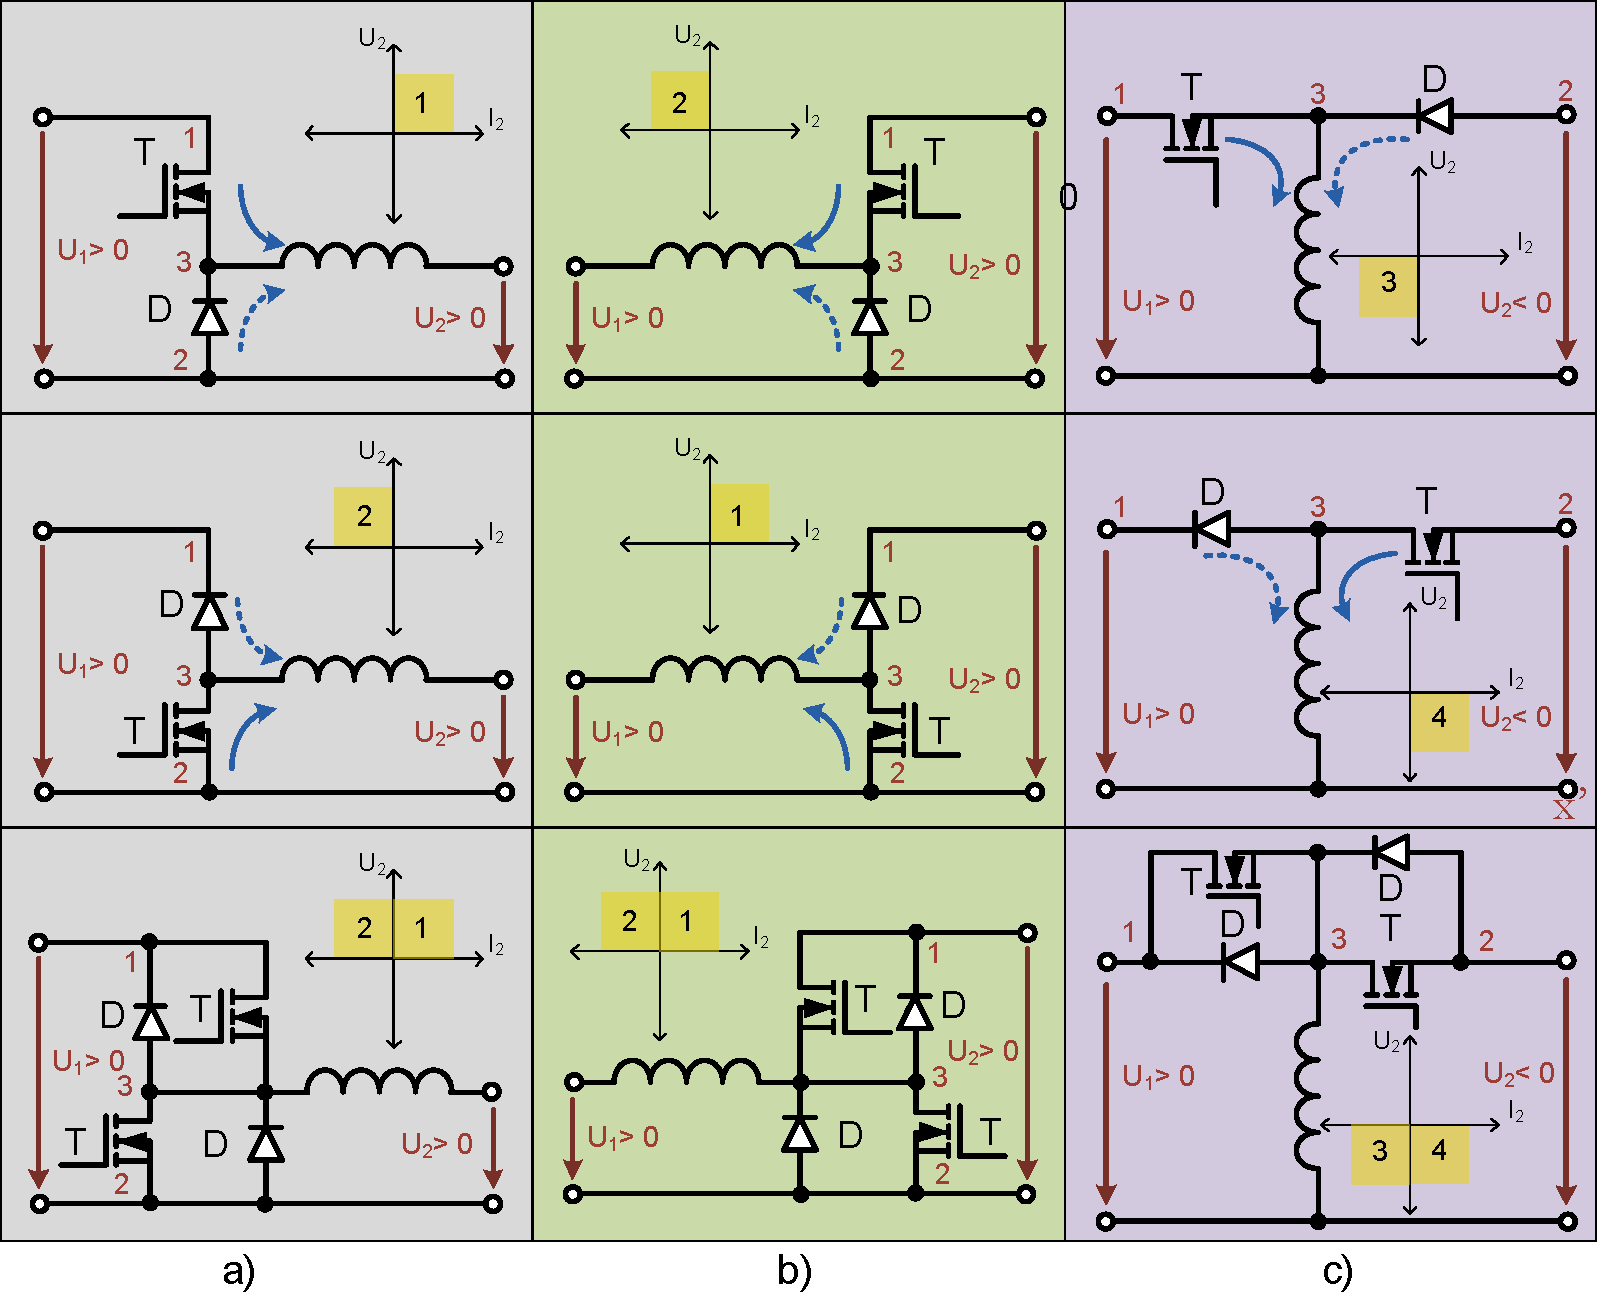
\includegraphics[width=0.9\linewidth]{aes_fig005.pdf}
          \caption[Skutečné silové obvody měničů a jejich kvadranty]{Skutečné silové obvody měničů
            z obr. \ref{enz:fig_002} a jejich pracovní kvadranty: a) měnič snižující
            neinvertující (step-down), b) měnič zvyšující neinvertující (step-up), c) měnič
            invertující (buck-boost)}
          \label{aes:fig005}
        \end{figure}

  %===== kapitola: DC/DC měniče bez transformátoru =================================================
  \section{Snižující neinvertující měnič}\label{aes:sec002}
    Jedná se o měnič s horním spínačem. Další jeho používané názvy jsou: propustný měnič, chopper,
    buck nebo step-down converter. \emph{Pracuje v 1. kvadrantu}.
    \begin{figure}[ht!] %\ref{enz:fig_003}
      \centering
      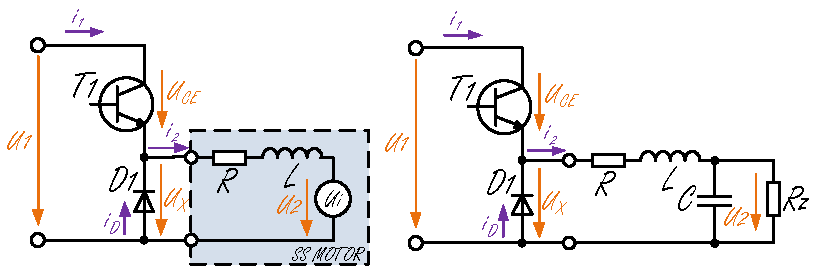
\includegraphics[width=0.8\linewidth]{patocka_step_down_sch1.pdf}
      \caption[Snižující měnič]{Snižující měnič pracující v prvním kvadrantu s aktivní zátěží
               typu stejnosměrný motor nebo s \texttt{LC} filtrem}
      \label{enz:fig_003}
    \end{figure}
    
    Schéma měniče a označení veličin je uvedeno na obr. \ref{enz:fig_003}. Na obr. 
    \ref{aes:fig002} jsou nakresleny průběhy veličin měniče s aktivní zátěží typu ss. motor s 
    cizím buzením - indukčnost \texttt{L} je kotevní indukčnost stroje. Na obr. \ref{aes:fig002b} 
    jsou průběhy měniče s \texttt{LC} filtrem pracující do zátěže \texttt{R\textsubscript{z}} 
    (např. nespojitý stabilizátor napětí).
  
    \begin{figure}[ht!]
      \centering
      \subcaptionbox{\label{aes:fig002a}}{\luafigure[0.3]{aes_fig002a.pdf}}
      \subcaptionbox{\label{aes:fig002b}}{\luafigure[0.3]{aes_fig002b.pdf}}
      \subcaptionbox{\label{aes:fig002c}}{\luafigure[0.3]{aes_fig002c.pdf}}
      \caption{Průběhy napětí a proudů snižujícího měniče}
      \label{aes:fig002}
    \end{figure}
    
    \subsection{Popis činnosti v \textbf{režimu spojitých proudů}}
    
      Režimem spojitých proudů rozumíme, že proud tlumivkou \texttt{L} nikdy během svého poklesu v 
      časovém intervalu \texttt{t\textsubscript{2}} neklesne na nulu a nesetrvává nulový. V mezním 
      případě se může dotknout nuly v jediném bodě, v okamžiku skončení doby 
      \texttt{t\textsubscript{2}}.
      \begin{enumerate}[noitemsep]
        \item Vyjdeme ze stavu, kdy tranzistor \texttt{T} je vypnutý. V ustáleném stavu měniče (tj. 
              po několika spínacích periodách) už teče tlumivkou \texttt{L} nenulový proud 
              \(i_2(t)\). Uzavírá se přes zátěž a nulovou diodu \texttt{D}. Ta je tedy otevřena a 
              napětí \(u_x\) je teď proto nulové (ve skutečnosti je mírně záporné: prahové napětí 
              diody v propustném směru). Zdrojem proudu v takto uzavřeném obvodu je indukčnost 
              \texttt{L}. Probíhá přechodový děj s časovou konstantou \(L/R\). Bude-li spínací 
              perioda (a tedy i doba vypnutí tranzistoru) dostatečně krátká, nestačí se během ní 
              změnit vnitřní napětí \(U_i\) motoru nebo napětí \(U_2\) zátěže s \texttt{LC} filtrem 
              a lze je považovat za konstantní. Proud \(i_2(t)\) tedy exponenciálně klesá se 
              zmíněnou časovou konstantou.
        \item Sepneme tranzistor \texttt{T}. Pak napětí \(u_x\) bude rovno \(U_1\). Dioda 
              \texttt{D} se proto uzavře a proud \(i_2(t)\) je dodáván ze zdroje \(U_1\). Opět 
              probíhá přechodový děj s časovou konstantou \(L/R\) - proud vzrůstá.
        \item Vypneme-li tranzistor, dostáváme se zpět do výchozího stavu 1.
      \end{enumerate}
      
      Kdyby odpor \texttt{R} byl roven \emph{nule}, změnily by se exponenciální průběhy proudu v 
      šikmé přímky (úsečky). V praxi je hodnota \texttt{R} opravdu velmi malá. Jde-li o zátěž ss. 
      motorem, je to jeho odpor vinutí, v případě \texttt{LC} filtru je to odpor vinutí tlumivky 
      \texttt{L}. Exponenciální průběhy se tedy budou šikmým přímkám velmi blížit. Provedeme tedy 
      zjednodušení a budeme uvažovat linearizované průběhy podle obr. \ref{aes:fig002b}.
      Přesně by tyto průběhy platily pro \(R = 0\). V případě nekonečně velké indukčnosti 
      \texttt{L} by proud \(i_2(t)\) musel být zcela konstantní, viz. obr. \ref{aes:fig002c}.
      
      \begin{tcnote}
        Povšimněme si zajímavé skutečnosti. Je-li zátěží měniče motor, není pozorovateli vůbec 
        fyzicky přístupno vyhlazené ss. napětí \(U_2\) (u motoru se jedná o vnitřní indukované 
        \(U_i\)), ale pouze impulsy \(u_x\) se střední hodnotou \(U_2\). Indukčnost stroje a zdroj 
        indukovaného napětí jsou vzájemně neseparovatelné. Hodnota \(U_i\) je určena otáčkami 
        motoru. Vidíme, že vlastní indukčnost motoru je užitečná. Kdyby neexistovala, museli bychom 
        použít samostatnou tlumivku vnější.
      \end{tcnote}
      
      Velikost napětí \(U_2\) byla odvozena v kapitole \ref{ENZ:tit_menice_s_1_aku_prvkem} a platí 
      pro ni vztah (\ref{aes:eq002}) - za předpokladu \(R = 0\). Zavedeme pojem \textbf{střída} 
      jako poměr doby zapnutí tranzistoru \(t_1\) a periody spínání \(T\).
      \begin{align}
        \delta &= \frac{t_1}{T} \qquad \delta\in(0, 1) \label{aes:eq001a} \\
        \shortintertext{Pak lze vztah (\ref{aes:eq002}) psát ve tvaru:}
        U_2    &= \delta\cdot U_1                      \label{aes:eq001b}
      \end{align}
    
      \subsubsection{Zvlnění výstupního proudu}
        Užijeme zmíněnou aproximaci průběhu proudů šikmými přímkami (tedy \(R = 0\)). V době 
        \(t_1\) (tranzistor sepnut) se proud\(i_2(t)\) zvýší o \(\Delta I\). Velikost zvlnění 
        souvisí s indukčností \(L\). Po dobu \(t_1\) je na indukčnosti konstantní napětí, dané 
        rozdílem \(U_1 − U_2\). Proto musí platit:
        \begin{align}
          U_1 - U_2 &= L\frac{\Delta I}{t_1}     \label{aes:eq003a} \\
          \shortintertext{Odsud plyne vztah pro \(\Delta I\):}
          \Delta I  &= \frac{(U_1 - U_2)t_1}{L}  \label{aes:eq003b} \\
          \shortintertext{Dosadíme za \(t_1\) z (\ref{aes:eq001a}) a \(U_2\) z (\ref{aes:eq001a}):}
          \Delta I  &= \frac{U_1(1 - \delta)\delta T}{L} 
                     = \frac{U_1(1 - \delta)\delta}{fL} \label{aes:eq003c} 
          \shortintertext{Kde \(f\) je pracovní kmitočet měniče.}
        \end{align}        
        Vidíme, že velikost zvlnění závisí na střídě. Hledáme maximum tohoto zvlnění. Derivujeme 
        tedy vztah (\ref{aes:eq003c}) dle \(\delta\) a derivaci položíme rovnu nule:
        \begin{equation}\label{aes:eq004}
          \der{(\Delta I)}{\delta} = \frac{U_1}{fL}(1-2s) = 0 
        \end{equation}
        Z rovnice (\ref{aes:eq004}) vidíme, že maximum nastává při \(\delta = \num{0.5}\). Po 
        dosazení \(\delta = \num{0.5}\) do vztahu (\ref{aes:eq003c}) dostaneme:
        \begin{equation}\label{aes:eq005}
          \Delta I_{max} = \frac{U_1}{4fL}  \qquad \delta =\num{0.5} 
        \end{equation}
        Z obr. \ref{aes:fig002b} je zřejmé, že maximální (tj. špičkový) proud tranzistoru i diody 
        je o \(\Delta I/2\) větší než střední hodnota \(I_2\). Proto nelze dovolit zvlnění proudu 
        velké, čili tlumivka s dostatečnou indukčností je nutná.
      
      \subsubsection{Napěťové dimenzování polovodičů}
        Tranzistor \texttt{T} je namáhán (ve vypnutém stavu) napětím \(U_1\), podobně dioda 
        \texttt{D} (při sepnutém tranzistoru). Při procesu zániku proudu tranzistorem (vypínání 
        tranzistoru) vzniká přídavný napěťový impuls na parazitní indukčnosti smyčky, tvořené 
        prvky: zdroj \(U_1\), tranzistor \texttt{T} a nulová dioda \texttt{D}. Velikost impulsu 
        závisí na velikosti proudu a na rychlosti vypínání (tedy na strmosti \(di/dt\)) a na
        velikosti zmíněné indukčnosti. Výsledkem je skutečnost, že oba prvky je nutno dimenzovat na 
        napětí rovné raději dvojnásobku \(U_1\). Pro omezení parazitní indukčnosti je nutné, aby 
        plocha zmíněné smyčky byla co nejmenší tj. zdroj \(U_1\), tranzistor a dioda musí být 
        umístěny co nejblíže u sebe. V praxi to znamená nutnost použít kvalitní, tzv. výkonový 
        impulsní bezindukční kondenzátor (svitkový, nejlépe s polypropylénovým dielektrikem) 
        umístěný paralelně k přívodům \(U_1\) - ale co nejtěsněji ke dvojici tranzistoru a diody.
        K omezení překmitů se také používají různé odlehčovací obvody. Ty mají kromě toho za úkol i
        omezení přepínacích ztrát tranzistoru.

      \subsubsection{Proudové dimenzování polovodičů}
        Zanedbáme-li pilovité zvlnění proudu \(i_C(t)\) tranzistorem a \(iD(t)\) diodou, lze určit 
        jejich špičkovou, střední a efektivní hodnotu pomocí vztahů (odvození - viz. obr  
        \ref{aes:fig002}):
        \begin{align}
          I_{C_{max}} &= I_2  \qquad  I_{C_{\text{stř}}} = I_2\cdot\delta    \qquad\qquad
                                I_{C_{ef}} = I_2\cdot\sqrt{\delta}       \label{aes:eq006a}   \\
          I_{D_{max}} &= I_2  \qquad  I_{D_{\text{stř}}} = I_2(1-\delta)     \qquad
                                I_{D_{ef}} = I_2\cdot\sqrt{1-\delta}     \label{aes:eq006b}
        \end{align}
        Všimněme si, že při velké střídě (tj. je velké výstupní napětí, blízké vstupnímu) je více 
        proudově namáhán tranzistor než nulová dioda a naopak. Tranzistor musí být volen tak, aby 
        špičkový proud \(I_{C_{max}}\) dle (\ref{aes:eq006a}) nepřesahoval jeho typový kolektorový 
        proud \(I_C\) (katalogový údaj). Čili je třeba dimenzovat tranzistor na tento špičkový 
        proud. Diodu pak dimenzujeme na proud střední dle (\ref{aes:eq006b}). Je třeba počítat vždy 
        s nejhorším možným režimem (\emph{střída}).
        
      \subsubsection{Ztrátový výkon polovodičů}
        \begin{itemize}
        \item \textbf{Ztráty vedením:} Sepnutý bipolární Darlington a tranzistor IGBT si lze 
              zjednodušeně představit (v omezeném rozsahu proudů) jako prvek s konstantním 
              saturačním napětím \(U_{CE_{sat}}\), nezávislým na procházejícím proudu.
              Tedy:
              \begin{equation}\label{aes:eq007}
                P_T = U_{CE_{sat}}\cdot I_{\text{stř}}
              \end{equation}
              Bipolární tranzistor (jednoduchý - ne Darlington) lze v sepnutém stavu přibližně 
              nahradit odporem, jehož hodnota je určena sklonem mezní přímky. U sepnutého 
              unipolárního výkonového tranzistoru \texttt{MOSFET} je přímo udávána hodnota odporu 
              \(R_{DS_{on}}\) v sepnutém stavu. Ztrátový výkon je tedy úměrný                 
              kvadrátu ef. hodnoty proudu:
              \begin{equation}\label{aes:eq008}
                P_T = R_{DS_{on}}\cdot I_{C_{ef}}^2
              \end{equation}
        \item \textbf{Přepínací ztráty tranzistoru:} Proces spínání a vypínání tranzistoru 
              neprobíhá nekonečně rychle, čili určitou dobu je tranzistor v aktivní oblasti, kdy na 
              něm vzniká velký okamžitý ztrátový výkon. Při jednom zapnutí se promění v teplo 
              energie \(W_{on}\), při jednom vypnutí \(W_{off}\). Ke stanovení těchto energií je 
              třeba přesnějšího rozboru přepínacích procesů v tranzistoru a v celém měniči. U 
              tranzistorů \texttt{IGBT} bývají tyto energie uváděny v podrobných katalozích: 
              \begin{equation}\label{aes:eq009}
                P_{\text{př}} = (W_{on} + W_{off})\cdot f
              \end{equation}
              Je tedy přímo úměrný pracovnímu kmitočtu měniče.
        \end{itemize}
        
        \begin{tcnote}
          Přídavné přepínací ztráty vznikají i na nulové diodě vlivem její nenulové zotavovací doby 
          \(t_{rr}\). Při procesu zapínání tranzistoru přebírá tranzistor postupně proud diody. 
          Teče-li již celý proud tranzistorem, mělo by to znamenat uzavření diody a skokový vzrůst 
          napětí \(u_x\) na ní z nuly na \(U_1\) (v závěrném směru). Dioda je však schopna po 
          jistou zotavovací dobu vést i proud opačného směru, je-li jí závěrné napětí \(U_1\) 
          příliš prudce vnuceno sepnutím tranzistoru. Vzniká tzv. \textbf{komutační zkrat}, 
          zkratový proud teče ze zdroje \(U_1\) přes tranzistor a „nezotavenou“ diodu. Tím dioda 
          zvyšuje ztráty tranzistoru a navíc na ní samotné vzniká vypínací ztrátový výkon.
        \end{tcnote}
      
      \subsubsection{Návrh filtračního kondenzátoru C}
        Kondenzátor \texttt{C} má zaručit, aby napětí na zátěži \texttt{R\textsubscript{z}}  bylo 
        téměř konstantní. To byl také předpoklad při odvozování průběhů proudů v měniči.
        
        \begin{tcnote}
          U zátěže motorové je konstantní hodnota \(U_i\) zaručena mechanickou setrvačností rotoru, 
          tj. momentem setrvačnosti stroje. U \texttt{LC} filtru 2. řádu, před zátěží 
          \texttt{R\textsubscript{z}}, je třeba zajistit setrvačnost elektricky tj.         
          kondenzátorem \texttt{C}. Bez jeho použití by napětí bylo filtrováno \texttt{LR} filtrem 
          1. řádu, tvořeným prvky \texttt{L} a \texttt{R\textsubscript{z}}. Zvlnění výstupního 
          napětí by ale bylo velké, resp. k jeho potlačení by bylo třeba příliš velké
          indukčnosti \texttt{L}. Navíc by zvlnění záviselo na velikosti 
          \texttt{R\textsubscript{z}}. Při impulsně proměnné zátěži v „mikroskopickém 
          vysokofrekvenčním“ smyslu (např. mikroskopicky nespojitý napájecí proud
          počítače), by napětí nabylo impulsního charakteru!
        \end{tcnote}
        
        \begin{figure}[ht!]
          \centering
          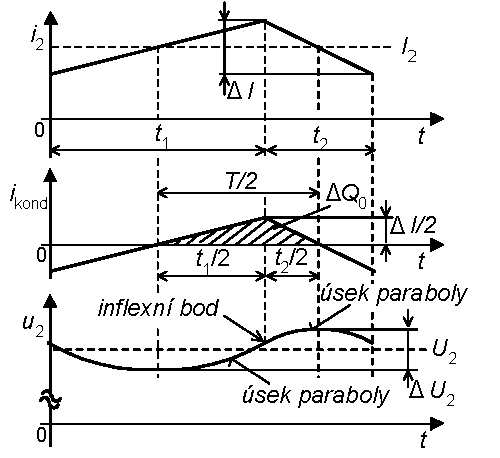
\includegraphics[width=0.8\linewidth]{aes_fig003.pdf}
          \caption{Vliv kondenzátoru \texttt{C} na průběh výstupního napětí \cite[s.~79]{Patocka}}
          \label{aes:fig003}
        \end{figure}
        Za předpokladu velmi malé konečné velikosti zvlnění výstupního napětí \(\Delta U_2 \ll 
        U_2\) (při použití \(C\)) lze tvrdit, že zátěží \texttt{R\textsubscript{z}} teče téměř 
        konstantní proud o velikosti \(I_2\). To znamená že výše odvozené zvlnění proudu \(\Delta 
        I_2\), čili jistá „střídavá složka“ proudu \(i_2(t)\) teče celá přes kondenzátor 
        \texttt{C}. Situace je na obr. \ref{aes:fig003}. Během doby, kdy má proud kondenzátorem 
        kladné znaménko, tj. kdy \(i_2(t) > I_2\), narůstá na kondenzátoru napětí. Náboj 
        kondenzátoru se během této doby zvětší o \(\Delta Q\), tj. o plochu vyšrafovaného 
        trojúhelníku v obr \ref{aes:fig003}, viz průběh \(i_{kond}(t)\):
        \begin{equation}\label{aes:eq012}
          \Delta Q   = \frac{\Delta I}{2}\frac{t_1+t_2}{4}=\frac{\Delta I}{8}T 
        \end{equation}
        
        \begin{align}
          \shortintertext{Napětí se během této doby zvětší o \(\Delta U_2\):}
          \Delta U_2 &= \frac{\Delta Q}{C} = \frac{\Delta I}{8C}T               \label{aes:eq013} \\
          \shortintertext{Pro požadované napěťové zvlnění \(\Delta U_2\) lze 
                          proto určit velikost \(C\):}
          C          &= \frac{\Delta I}{\Delta U}\frac{T}{8}                    \label{aes:eq014} \\
          \shortintertext{Přitom za \(\Delta I\) můžeme dosadit výše 
                          uvedený vztah (\ref{aes:eq005}) a dostaneme:}
          C          &= \frac{U_1(1-\delta)\delta}{8Lf^2\Delta U_2}             \label{aes:eq015}
        \end{align}
        
        \begin{tcnote}
         Kapacitu \(C\) je nutno realizovat pomocí výkonového impulsního elektrolytického 
         kondenzátoru s malým sériovým vnitřním odporem (malý činitel \(\tan\delta\)) a paralelně 
         zapojeným bezindukčním impulsním svitkovým kondenzátorem (nejlépe s polypropylénovým 
         dielektrikem). Je možné nouzově použít i sadu mnoha „obyčejných“ elektrolytických 
         kondenzátorů spojených paralelně, čímž minimalizujeme vni\-třní sériový odpor i sériovou 
         indukčnost. Tato indukčnost jinak výrazně degraduje filtraci, zvláště při vyšších 
         kmitočtech. Sériový odpor je vedle degradace filtrace také navíc příčinou tepelných ztrát 
         na kondenzátoru. Použití jediného obyčejného elektrolytického kondenzátoru byť s 
         dostatečnou kapacitou \(C\) je pak skoro bezcenné a může být i nebezpečné (exploze po 
         přehřátí).
        \end{tcnote}
      
        Na závěr je nutné zkontrolovat, zdali vlastní rezonanční kmitočet obvodu \texttt{LC} leží 
        dostatečně nízko pod  pracovním kmitočtem měniče \(f\). Tedy musí platit:
        \begin{equation}\label{aes:eq016}
          C\gg\frac{1}{4\pi^2f^2L}
        \end{equation}
        
    \subsection{Popis činnosti v režimu přerušovaných proudů}
      Princip činnosti je stejný jako v \emph{režimu spojitých proudů}. Střední hodnota proudu 
      \(I_2\) je však tak malá, že někdy během doby \(t_2\) (kdy je tranzistor vypnutý a setrvačný 
      proud tlumivky \texttt{L} klesá), klesne proud až na nulu, dříve než doba \(t_2\) skončí. V 
      tom okamžiku se zavře dioda \texttt{D} a v měniči pak nevede ani tranzistor ani dioda - čili 
      zátěž je zcela odpojena. Proto se na svorkách \(U_x\) objeví vnitřní napětí zátěže
      (buď \(U_i\) motoru, nebo \(U_2\) \texttt{LC}-filtru). To je možné proto, že indukčností 
      \texttt{L} (motoru nebo tlumivky) neteče v této situaci žádný proud, tedy je nulové také 
      \(di/dt\) čili i napětí na \texttt{L}. Indukčnost \texttt{L} lze v takové situaci nahradit 
      „drátem“. Tento stav trvá až do okamžiku sepnutí tranzistoru \texttt{T}, kdy začne být 
      \(u_x(t)\) rovno \(U_1\).
      
      Z obr. \ref{aes:fig004} je vidět, že v režimu přerušovaných proudů popisovaný jev zvyšuje 
      střední hodnotu napětí \(u_x\), což je hodnota výstupního napětí, uvažujeme-li \(R = 0\). 
      Výstupní napětí bude tedy vyšší než  udává vztah (\ref{aes:eq001a}) pro režim spojitých 
      proudů.
      
      \begin{figure}[ht!]
        \centering
        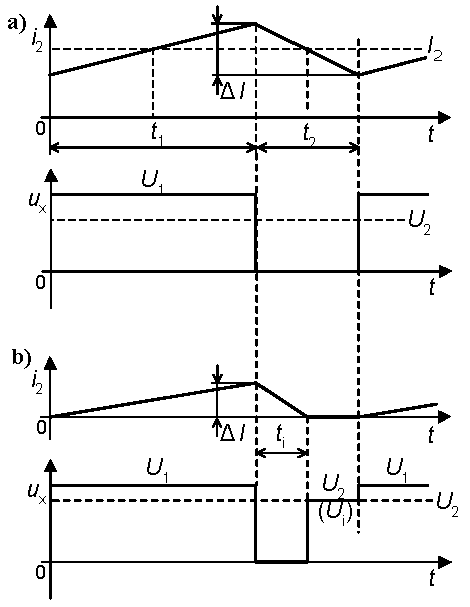
\includegraphics[width=0.8\linewidth]{aes_fig004.pdf}
        \caption{Proud a napětí zátěže u měniče step-down: a) režim spojitých proudů
                 b) režim přerušovaných proudů}
        \label{aes:fig004}
      \end{figure} 
      Růst napětí na kondenzátoru \texttt{LC}-filtru je výsledkem vzájemné energetické interakce 
      mezi vstupním zdrojem, tlumivkou, kondenzátorem a zátěží. Jev lze vysvětlit takto:
      Vyjděme ze situace, že zátěž je zcela odpojena a výstupní proud je tedy nulový. Pak 
      dlouhodobě, v ustáleném stavu, musí být zcela nulový i proud tekoucí tlumivkou \texttt{L}. 
      Toho lze však docílit jedině tak, že v době sepnutí tranzistoru bude na tlumivce nulové 
      napětí. Neboli, před i za tlumivkou bude stejně velké napětí, tedy musí platit \(U_2 = U_1\). 
      Ve stavu zcela \emph{naprázdno} tedy výstupní napětí vzroste na \emph{maximální} možnou 
      hodnotu \(U_1\) a to bez ohledu na střídu, s jakou měnič pracuje.
      
      Stejnosměrný proud zátěže musí být roven střední hodnotě proudu tlumivky (střední hodnota 
      kapacitního proudu musí být totiž nulová). Pak bude-li ss. proud zátěže nenulový, ale velmi 
      malý, musí být velmi malá hodnota středního proudu tekoucího tlumivkou. Toho lze dosáhnout 
      pouze režimem přerušovaných proudů. Ten může ale nastat pouze tehdy, změní-li se strmosti 
      \(di/dt\) náběžné a sestupné části trojúhelníkovitého průběhu proudu oproti režimu spojitému. 
      Změna strmostí di/dt může být dosažena pouze změnou napěťových poměrů na tlumivce. Tzn., že 
      klesá-li plynule střední hodnota přerušovaných proudů k nule, musí současně plynule růst 
      výstupní napětí na hodnotu \(U_1\).

  \section{Zvyšující neinvertující měnič}\label{aes:sec006}
    Jedná se o měnič z obr. \ref{aes:fig005}b), varianta s dolním spínačem. Jeho další název je: 
    \textbf{boost converter}. Jak už bylo uvedeno v kap. \ref{aes:sec001} je tento měnič pracující 
    v 1.  kvadrantu \emph{ekvivalentní měniči step-down pracujícímu ve 2. kvadrantu}, obr. 
    \ref{aes:fig005}a), s dolním spínačem, pouze zátěž a zdroj si vyměnily své role.
    Schéma zapojení a průběhy důležitých veličin jsou na obr. \ref{aes:fig006}. Průběhy proudů jsou 
    opět aproximovány šikmými přímkami, takže zavádíme předpoklad nulového odporu ve smyčce tlumivky
    (viz. kap. \ref{aes:sec002}).
    
    \begin{figure}[h!]
      \centering
      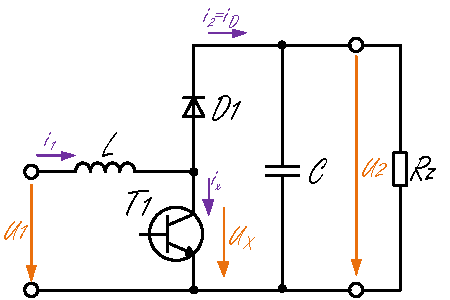
\includegraphics[width=0.5\linewidth]{aes_fig006.pdf}
      \caption{Zvyšujícího měnič pracující v prvním kvadrantu - Schéma zapojení}
      \label{aes:fig006}
    \end{figure}
    \begin{tcnote}
      Má-li být výstupní napětí \(U_2\) konstantní, je nutno použít filtrační sběrný kondenzátor 
      \texttt{C}. Zátěž měniče tedy nemá induktivní charakter. Naopak přítomnost indukčnosti 
      \texttt{L} zapojené v sérii se vstupním napěťovým zdrojem je nezbytná. Vstupní zdroj s 
      indukčností \texttt{L} může být nahrazen aktivní zátěží tj. např. motorem pracujícím v 
      generátorickém režimu. Pak je indukčnost \texttt{L} součástí motoru, jakožto jeho
      vlastní indukčnost a v topologii měniče není explicitně vyjádřena. Stejnosměrné vstupní 
      napětí \(U_1\) je potom vnitřním napětím \(U_i\) a v režimu spojitých proudů není fyzicky 
      měřitelné, neboť svorkami motoru jsou svorky \(u_x\).
    \end{tcnote}
    
    \subsection{Popis činnosti v režimu spojitých proudů}
      „Spojitost“ a „nespojitost“ se týká opět proudu tlumivkou, tj. u tohoto měniče jde o proud 
      vstupní \(i_1(t)\).
      \begin{enumerate}[noitemsep]
        \item Tranzistor \texttt{T} je vypnutý. V ustáleném stavu (po několika spínacích periodách) 
              už teče tlumivkou \texttt{L} určitý proud ze zdroje \(U_1\) přes \texttt{D} do zátěže 
              \(U_2\). Dioda \texttt{D} je tedy otevřená. Na tlumivce \texttt{L} je proto napětí 
              \(u_L = U_1 − U_2\). Je záporné, protože \(U_2 > U_1\). Proto proud tlumivkou 
              lineárně klesá.
        \item Sepneme-li tranzistor, objeví se na tlumivce kladné konstantní napětí \(u_L = U_1\) a 
              proud \(i_1\), tekoucí tlumivkou, začne lineárně narůstat. Uzavírá se přitom ze 
              zdroje \(U_1\) přes \texttt{L} a tranzistor. Dioda \texttt{D} je polarizována v 
              závěrném směru a je uzavřená.
        \item Vypnutím tranzistoru se dostáváme do výchozího stavu 1).
      \end{enumerate}
      
      V kap \ref{aes:sec001} jsme odvodili vztah (\ref{aes:eq016}) pro velikost \(U_2\). Při 
      uvažování pojmu střída dle vztahu (\ref{aes:eq001a}) lze vztah (\ref{aes:eq016}) přepsat do 
      podoby:
      \begin{equation}
        U_2 = U_1 \frac{t_1 + t_2}{t_2} = U_1\frac{T}{t_2} = U_1\frac{1}{1-\delta}
      \end{equation}
      Je zřejmé, že \(U_2\) musí být větší než \(U_1\). Kdyby tomu tak nebylo, tak by při vypnutém 
      tranzistoru nebylo napětí \(u_L\) záporné a proud \(i_1\) by nemohl klesat. Narůstal by tedy 
      nejen v době, kdy je tranzistor sepnutý, ale i v době, kdy je vypnutý a rostl by tedy nade 
      všechny meze.
      
      \subsubsection{Zvlnění vstupního proudu}
        V době \(t_1\) (tranzistor \texttt{T} sepnut) se proud \(i_1(t)\) zvýší o \(\Delta I\). V 
        době \(t_2\) se o tutéž velikost sníží. Velikost \(\Delta I\) určíme např. pomocí doby 
        \(t_1\). Během ní je na tlumivce \texttt{L} napětí \(U_1\). Musí proto platit:
        \begin{align}
          U_1 &= L\frac{\Delta I}{t_1} \label{aes:eq022}  \\
          \shortintertext{Za \(t_1\) dosadíme vztah (\ref{aes:eq001a}) a vyjádříme \(\Delta I\):}
          \Delta I &= \frac{U_1\delta T}{L} = \frac{U_1\delta }{fL}  \label{aes:eq023}
        \end{align}
        Velikost zvlnění opět závisí na střídě. Je zřejmé, že maximální zvlnění nastane při 
        maximální střídě (blízké jedné).
        
      \subsubsection{Napěťové dimenzování polovodičů}
        Tranzistor \texttt{T} je namáhán napětím \(U_2\) (je-li vypnut a tedy dioda \texttt{D} 
        otevřena). Podobně dioda je namáhána tímtéž napětím \(U_2\) při sepnutém tranzistoru. 
        Napěťové namáhání polovodičů roste při zvyšování střídy (roste \(U_2\)). Pozor, podle 
        (\ref{aes:eq022}), pro \(\delta\rightarrow1\) roste výstupní napětí nade všechny meze.
        Opět u tohoto měniče nastávají navíc problémy s přepěťovými špičkami na parazitních 
        indukčnostech, které byly popsány v kap. \ref{aes:sec002} u měniče snižujícího.
        
      \subsubsection{Proudové dimenzování polovodičů}
        Zanedbáme-li pilovité zvlnění proudu \(i_C(t)\) tranzistorem a \(i_D(t)\) diodou, lze určit 
        jejich špičkovou, střední a efektivní hodnotu pomocí následujících vztahů (viz. obr. 
        \ref{aes:fig006}):

    \subsection{Popis činnosti v režimu přerušovaných proudů}

  \section{Invertující měnič se společnou tlumivkou}\label{aes:sec003}  
    Jedná se o měnič z obr. \ref{aes:fig005}c), varianta s horním spínačem. Jeho další názvy jsou: 
    \emph{buck-boost}, blokující měnič. Měnič pracuje ve 3. kvadrantu. Schéma měniče a důležité 
    průběhy napětí a proudů jsou na obr. \ref{enz:fig_007}.
    
    Šipka napětí \(U_2\) je vyznačena s ohledem na skutečnou polaritu tohoto výstupního napětí, na 
    rozdíl od obr. \ref{aes:fig005}, kde jsme pak museli uvažovat napětí \(U_2\) záporné.
    
    \begin{figure}[ht!]
      \centering
      \subcaptionbox{\label{enz:fig_007a}}{\luafigure[0.45]{patocka_buckboost_sch.pdf}}
      \subcaptionbox{\label{enz:fig_007b}}{\luafigure[0.45]{patocka_buckboost_pr.pdf}}
      \caption{Invertující měnič pracující ve 3. kvadrantu: a)schéma zapojení b) průběhy napětí a 
               proudů}
      \label{enz:fig_007}
    \end{figure}
    
    \begin{tcnote}
      Kondenzátor C zapojený mezi vstup a výstup (kresleno čárkovaně) není principiálně nutný, 
      neboť i bez něj je napětí mezi vstupem a výstupem konstantní a je dáno součtem konstantního 
      \(U_1\) a napětí \(U_2\). \(U_2\) je téměř konstantní při dostatečné velikosti CZ.
      
      Kondenzátor C je ale nutný v případě, kdy CZ není použit a zátěž má induktivní charakter 
      (např. jde o motor). Na její indukčnosti by pak vznikaly nekontrolovatelné napěťové špičky 
      díky impulsnímu charakteru proudu \(i_2(t)\) - viz. obr. \ref{enz:fig_007b}). Tyto špičky by 
      napěťově zničily polovodiče měniče.
    \end{tcnote}
    
    Průběhy proudů jsou opět aproximovány šikmými přímkami, takže znovu zavádíme předpoklad
    nulového odporu ve smyčce tlumivky L, viz. kap. 8.6.
    
    Popis činnosti v režimu spojitých proudů:
    \begin{itemize}
      \item Tranzistor T je vypnutý. V ustáleném stavu měniče (po několika spínacích periodách) už 
            teče tlumivkou L určitý proud iL. Uzavírá se přes zátěž a diodu D. Ta je tedy otevřená 
            a napětí \(u_x\) je tak rovno napětí \(U_2\). Na cívce L je tedy konstantní napětí 
            opačné polarity než má procházející proud. Ten proto lineárně klesá.
      \item Sepneme-li tranzistor T, je napětí \(u_x\) rovno napětí \(U_1\). Na cívce L je tedy 
            konstantní napětí \(U_1\). Proud proto lineárně narůstá. Uzavírá se tentokrát ze zdroje 
            \(U_1\) přes tranzistor. Dioda D je polarizována v závěrném směru a proud \(i_2(t)\) 
            neteče.
      \item Vypnutím tranzistoru se dostáváme do výchozího stavu 1).
    \end{itemize}
    
    V kapitole 8.5.1 jsme odvodili vztah (8.7) pro velikost U2. Zavedením pojmu střída dle vztahu 
    (8.8) a neuvažováním záporného znaménka (máme nyní opačně označenou šipku U2) lze (8.7) upravit 
    do podoby:
    
  \section{Čukův měnič}\label{aes:sec004}
    Tento měnič pracuje ve \emph{3. kvadrantu}. Používá ke své činnosti vedle dvou akumulačních 
    tlumivek ještě další akumulační prvek - \emph{kondenzátor} (měnič se společným kondenzátorem). 
    Nepatří tedy už do skupiny nejjednodušších měničů, které jsou na obr. \ref{aes:fig005}. Stále 
    pro něj však platí pravidla popsaná v kapitole \ref{aes:sec012} a způsob realizace „přepínače“ 
    popsaný v kapitole \ref{aes:sec001}. Čukův měnič pracující ve 3. kvadrantu pak obsahuje horní 
    spínač.
    
  \section{Měnič SEPIC}\label{aes:sec011}


  %--------------------- Kapitola: DC/DC měniče s transformátorem ----------------------------------
  \section{DC/DC měniče s transformátorem}\label{aes:sec007}
    Základní popis DC/DC měničů bez transformátoru, lze aplikovat i na měniče s transformátorem. 
    Doplněním vhodně zapojeného vf. impulsního transformátoru je umožněno galvanické oddělení 
    výstupního a vstupního napětí a transformaci napětí a proudů. Nejčastěji se v praxi setkáme s 
    transformátorovými verzemi měniče propustného z kap. \ref{aes:sec002} a měniče 
    blokujícího z kap.\ref{aes:sec006} Existuje i transformátorová verze měniče Čukova z kap. 
    \ref{aes:sec004}.
  
    Snižující měnič z kap \ref{aes:sec002} je v transformátorové verzi nazýván výhradně jako
    \textbf{měnič propustný}, neboť díky transformátoru lze převodovým poměrem zajistit výstupní 
    napětí i vyšší než vstupní (názvy „\emph{snižující měnič}“ a „\emph{step-down}“ by tedy byly 
    zavádějící). Princip činnosti však v hrubých rysech zůstává stejný.
  
    Invertující měnič se společnou tlumivkou z kap. \ref{aes:sec003} je v transformátorové 
    verzi nazýván výhradně jako \textbf{měnič blokující}, neboť díky transformátoru lze vyrobit 
    napětí libovolné polarity (název „\emph{invertující měnič}“ proto pozbývá výstižnosti).
  
    Základní stavební kameny měničů bez transformátoru tj. horní spínač a dolní spínač (kap.
    \ref{aes:sec001}) tvoří základ i u měničů s transformátorem, i když v zapojeních 
    jsou tranzistor a jeho protilehlá dioda \emph{rozděleny} tím, že je tranzistor na primární 
    straně a dioda na sekundární. Použití transformátoru navíc vyžaduje demagnetizační obvody 
    (zajištění nulové střední hodnoty primárního napětí) a další výstupní usměrňovací diodu 
    (diody). To vše vede k tomu, že transformátorové měniče jsou \emph{jednokvadrantové}. Výstupní 
    napětí má jedinou možnou polaritu a výstupní proud jediný možný směr takový, že zátěž se chová 
    vždy jako spotřebič, nikoli jako generátor.

    %------------- Jednočinný propustný měnič - základní zapojení ----------------------------------
    % !TeX spellcheck = cs_CZ
\section{Jednočinný propustný měnič}\label{ENZ:ssec_03}\hypertarget{ENZ:ssec_03} 
  Propustné měniče se vyznačují tím, že energie je přenášena ze vstupu na výstup v době zapnutí 
  tranzistoru, nikoli v době vypnutí, jak je tomu u měničů blokujících.
  
  V této i v následujících kapitolách budou analyzovány měniče typu DC/DC, které obsahují 
  vysokofrekvenční impulzní transformátor na feritovém jádře. Transformátor zajišťuje galvanické 
  oddělení mezi vstupní a výstupní stranou měniče. Je-li vstupní stejnosměrné napětí získáno 
  usměrněním střídavé sítě, pak bývají tyto měniče někdy označovány jako tzv. \emph{síťové 
  spínané 
  zdroje}.
  
  Celý výkonový řetězec sestává z následujících základních bloků:
  \begin{itemize}[noitemsep]
    \item buď síťový usměrňovač - stejnosměrný meziobvod - vlastní měnič,
    \item nebo akumulátor - stejnosměrný meziobvod - vlastní měnič.
  \end{itemize}
  
  Stejnosměrný meziobvod (ss. mezilehlý obvod, DC-bus, zwischenkreis) bývá napěťového typu, tj. 
  vůči následujícímu měniči se chová jako (téměř) ideální zdroj konstantního napětí \(U_d\) 
  nulovou vnitřní impedancí. Bývá realizován buď LC-filtrem, nebo samostatným sběracím 
  kondenzátorem o velké kapacitě. Dvojcestným usměrněním sítě 1 x \qty{230}{\volt} vznikne na 
  sběracím kondenzátoru ss. mezilehlé napětí \(U_d\) o hladině přibližně \qty{300}{\volt}. 
  Šestipulsním usměrněním sítě 3 x \qty{400}{\volt} vznikne ss. napětí o jmenovité střední hodnotě 
  \qty{542}{\volt}.
  
  Na hladině \qty{542}{\volt} se obvykle používají tranzistory IGBT se závěrným napětím 
  \qty{1200}{\volt}, které pracují na spínacím kmitočtu od \qty{25}{\kilo\hertz} do 
  \qty{60}{\kilo\hertz} (podle přenášeného výkonu). Kmitočet je ve většině případů omezen 
  především přepínacími ztrátami v tranzistorech IGBT.
  
  Na hladině \qty{300}{\volt} bývají převážně používány tranzistory MOSFET se závěrným napětím 
  \qty{600}{\volt}. Tranzistory jsou v současnosti tak rychlé, že mohou pracovat na spínacím 
  kmitočtu až do \qty{300}{\kilo\hertz}. Pracovní kmitočet ležívá typicky v oblasti 
  \qty{40}{\kilo\hertz} až \qty{120}{\kilo\hertz}. Jediným důvodem ke zvyšování kmitočtu je 
  zmenšování objemu transformátoru i výstupní tlumivky. Zvyšování kmitočtu nad 
  \qty{200}{\kilo\hertz} není výhodné z následujících důvodů:
  \begin{itemize}[noitemsep]
    \item Mezní kmitočet manganato-zinečnatých feritů leží kolem \qty{450}{\kilo\hertz}, tudíž 
          v pásmu nad \qty{200}{\kilo\hertz} prudce rostou hysterezní ztráty (viz komplexní 
          permeabilita v kap. 6.4.4.). Ztráty je nutno omezovat snižováním maximální pracovní 
          indukce \(B_{max}\), což působí proti zmenšování transformátoru.
     \item V oblasti nad \qty{200}{\kilo\hertz} začínají narůstat problémy se skinefektem ve  
          vinutí transformátoru (nikoli ve vinutí tlumivky, v ní je proud téměř hladký). Na 
          kmitočtu \qty{200}{\kilo\hertz} činí hloubka vniku již pouze \(\delta\cong\) 
          \qty{0,14}{\mm}, viz kap. 4. Nutné je použití vf. lanka nejen na sekundám (málo závitů a 
          velký průřez), ale i na primáni (více závitů a menší průřez). Výsledkem je pokles 
          činitele plnění ve vinutí, který působí proti zmenšování transformátoru.
    \item S rostoucím pracovním kmitočtem/dramaticky roste reaktance \(2\pi f L_{2,K}\) 
          výstupní rozptylové indukčnosti transformátoru \(L_{2,K} = L2(1 - k^2)\). Transformátor 
          je pak velmi měkký a není schopen přenést požadovaný výkon. Jedinou obranou je dosažení 
          co největšího činitele vazby \(k\). Hodnota \(k = 0,990\) je naprosto nedostatečná. 
          Nutným minimem bývá \(k = 0,998\), což ale přináší značné konstrukční problémy (viz 
          kap. 17.6).
    \item S rostoucím kmitočtem roste negativní vliv parazitních mezizávitových kapacit vinutí.
  \end{itemize}
  
  \subsection{Můstkový jednočinný propustný měnič - základní zapojení}
    Základní zapojení jednočinného propustného měniče s transformátorem je nakresleno na obr. 
    \ref{enz:fig_fey_1cinprop_m}. Jak již bylo předesláno, k přenosu energie ze vstupního do 
    výstupního obvodu dochází v aktivním intervalu \(0\) až \(\delta T\), během něhož se současně 
    akumuluje energie v magnetickém poli tlumivky \(L\). Po dobu zbývající části periody 
    $(1-\delta)T$ je tlumivka od transformátoru oddělena a na výstup dodává energii nahromaděnou  
    v magnetickém poli. Vzhledem k \emph{blokujícímu měniči} je zde výhoda účinného LC filtru 
    tvořeného tlumivkou a výstupním kondenzátorem \(C\) po dobu celého pracovního cyklu. Ve 
    srovnání s blokujícím měničem je tedy možné dosáhnout řádově menší dynamické odchylky 
    \(\Delta U_z(t)\). Navíc proud tekoucí \(L\), skládající se z ustálené složky $I_z$ a 
    pilovitého průběhu $\Delta i_L$ má spojitý charakter v průběhu celé periody $T$. 
    
    Časové průběhy všech důležitých veličin jsou zachyceny na obr. \ref{enz:fig_fey_1cinprop_mw}. 
    Z důvodu snadnějšího výkladu budeme při prvotní analýze předpokládat následující zjednodušení:

    \begin{itemize}[noitemsep]
      \item Tlumivka výstupního LC-filtru má velikou (nekonečnou) indukčnost. Proud tlumivky  
            \(i_L\) je hladký, málo zvlněný, tudíž je přímo roven proudu zátěže: \(i_L(t) = I_Z = 
            \text{konst}\).
      \item Transformátor má dokonalou magnetickou vazbu \(k=1\). Neexistuje tedy výstupní 
            rozptylová indukčnost \(L_{2,K}\).
    \end{itemize}
    Obě zjednodušení později při detailní analýze odstraníme.
    
    \begin{figure}[ht!]
      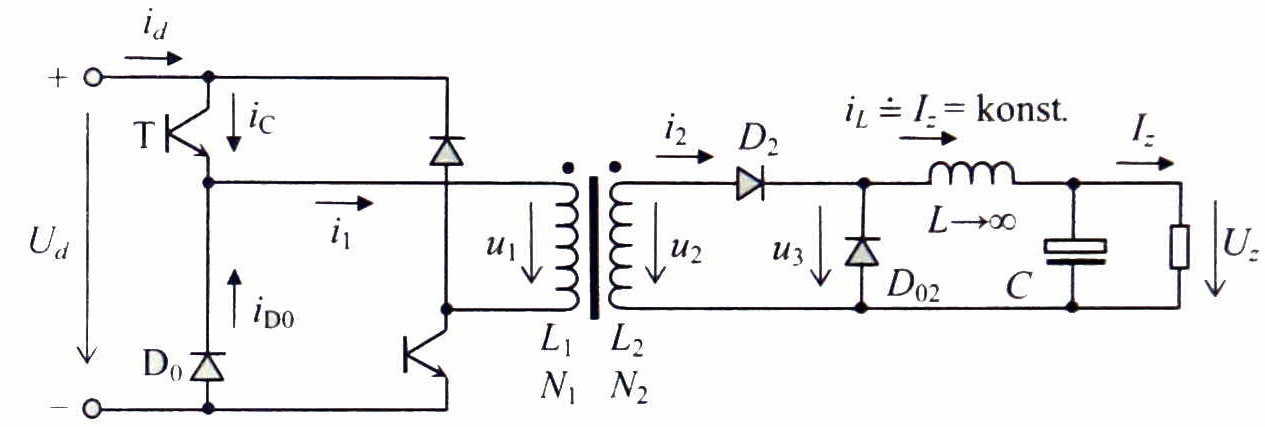
\includegraphics[width=\linewidth]{patocka_1cinprop_menic.JPG}
      \caption{Jednočinný propustný měnič - základní zapojení}
      \label{enz:fig_fey_1cinprop_m}
    \end{figure}
  
    Měnič pracuje tak, že oba tranzistory jsou vždy zapínány i vypínány současně. Doba zapnutí je 
    označena \(t_z\). Střída je definována vztahem
    \begin{equation}\label{enz:eq_1cinpropm01}
      s = \frac{t_z}{T}, \qquad s_{max} = \frac{1}{2}, \qquad \text{protože} \qquad t<\frac{T}{2}
    \end{equation}     

    \begin{figure}[ht!]
      \centering
      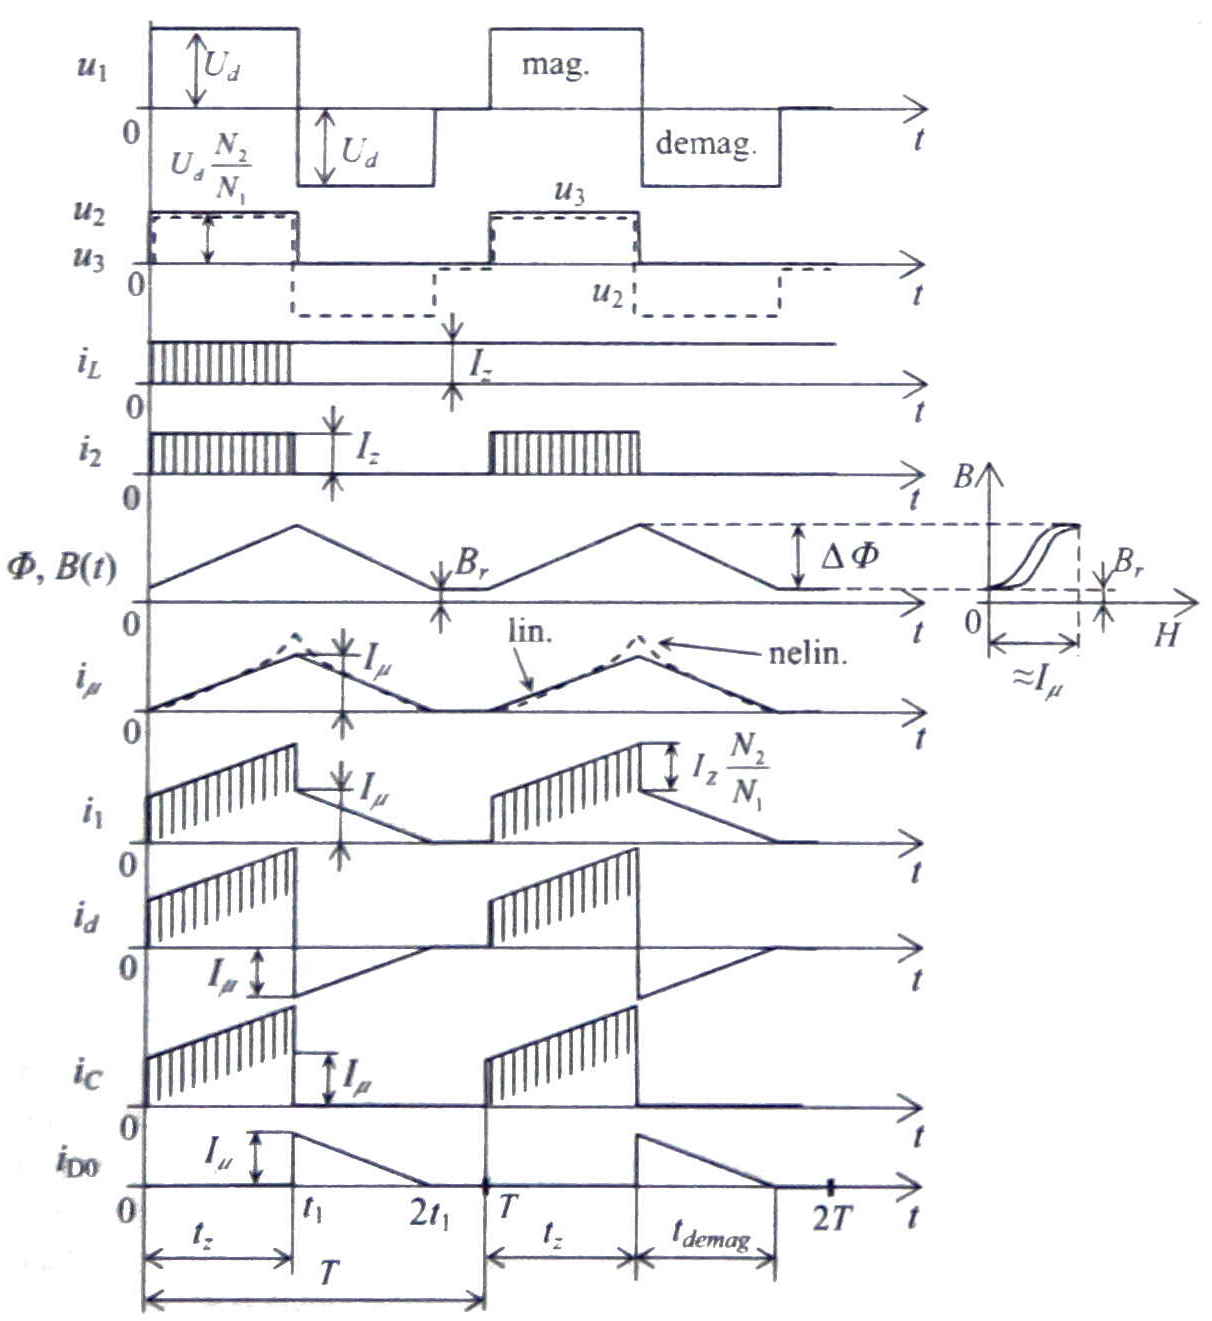
\includegraphics[width=\linewidth]{patocka_1cinprop_menic_w.JPG}
      \caption{Jednočinný propustný měnič - průběhy důležitých veličin.}
      \label{enz:fig_fey_1cinprop_mw} 
    \end{figure}
    
    Maximální doba zapnutí \(t_z=t_1\), nesmí překročit hodnotu \(\dfrac{T}{2}\), neboť pak 
    dochází k lavinovitému přesycení transformátoru podle obr. \ref{enz:fig_fey_1cinprop_syc}. 
    Při zapnutí obou tranzistorů má primární napětí konstantní hodnotu \(U_1(t)=+U_d\). 
    Magnetizační proud je integrálem z tohoto \emph{konstantního} napětí, proto narůstá 
    \emph{lineárně} (pokud zanedbáme nelinearitu magnetizační charakteristiky). V okamžiku 
    \(t_1\) jsou oba tranzistory vypnuty. Magnetizační indukčnost \(L_1\), však nedovolí zánik 
    magnetizačního proudu a snaží se jej udržet na původní velikosti. Proud tedy musí začít téci 
    oběma primárními diodami. Přes obě sepnuté diody připojí primární vinutí samo sebe na 
    napájecí zdroj \(U_d\) ale v opačné polaritě, tedy bude \(U_1(t)=-U_d\). Tímto napětím je 
    jádro \emph{demagnetováno} a magnetizační proud klesá, protože integrál ze záporné konstanty 
    je klesající přímka. Obě diody se uzavřou až v okamžiku zániku magnetizačního proudu. Teprve 
    tehdy je primární vinutí zcela odpojeno od mezilehlého zdroje \(U_d\), stává se neutrálním 
    vodičem neobsahujícím energii, proto teprve tehdy klesne primární napětí na nulu.
    
    Sekundární napětí \(u_2\) musí mít \emph{stejný tvar} jako napětí \(u_1\), pouze je s 
    převodem jinak velké. Záporný demagnetizační puls nesmí být využit k přenosu energie. Došlo 
    by k narušení procesu demagnetizace. Proto musí být na sekundáru použit pouze jednocestný 
    usměrňovač \(D_2\) s nulovou diodou \(D_{02}\) (nikoli dvojcestný). Dioda \(D_{02}\) vede 
    proud tlumivky v době, kdy jsou oba tranzistory vypnuty, a usměrňovači dioda \(D_2\) je 
    polarizována v závěrném směru. Užitečné napětí \(u_3\), na vstupu LC-filtru má potom tvar 
    jednopolaritních impulsů o maximální střídě 0,5.
    
    Sekundární proud \(i_2\) má podobu \emph{pravoúhlých} proudových impulsů, protože pokud proud 
    sekundárem teče, tlumivka s velikou indukčností \((L\rightarrow\infty)\) jej udržuje 
    \emph{konstantní}. S ohledem na vysoký pracovní kmitočet a na velký obsah harmonických je 
    nutno učinit velmi přísná opatření proti vzniku skinefektu. Z toho důvodu nesmí být průměr 
    sekundárního vodiče nebo tloušťka měděné fólie větší než \(2\delta\), kde \(\delta\) je 
    hloubka vniku. Totéž platí i o primárním vodiči.


    \begin{figure}[ht!]
      \centering
      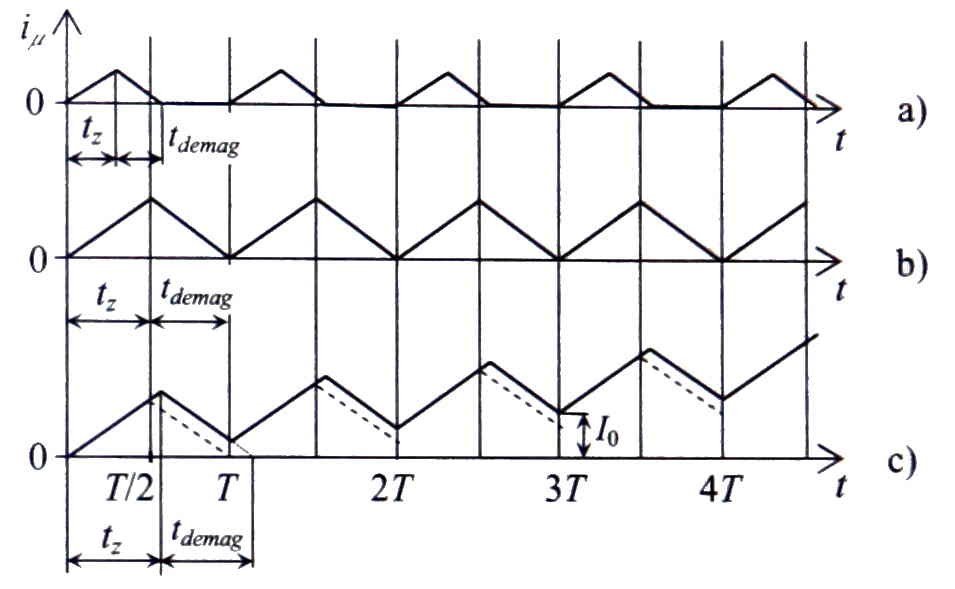
\includegraphics[width=0.8\linewidth]{patocka_1cinprop_syceni.JPG}
      \caption{Demagnetizace transformátoru při různých dobách zapnutí \(t_z\): a) dobrý stav 
               \(t_z < \frac{T}{2}\), b) mezní stav \(t_z = \frac{T}{2}\), c) špatný stav \(t_z > 
               \frac{T}{2}\)}.
      \label{enz:fig_fey_1cinprop_syc}
    \end{figure}
    Maximální doba zapnutí \(t_z=t_1\), nesmí překročit hodnotu \(\dfrac{T}{2}\), neboť pak 
    dochází k lavinovitému přesycení transformátoru podle obr. \ref{enz:fig_fey_1cinprop_syc}.  
    Jev je způsoben tím, že doby magnetizace a demagnetizace jsou stejně dlouhé, tj. 
    \(t_z=t_{demag}\). Demagnetizační proud proto zaniká v okamžiku \(2t_z\). Pokud v případě c) 
    doba zapnutí překročí \(\dfrac{T}{2}\), tj. \(2t_z > T\), magnetizační proud nestihne v rámci 
    pracovního cyklu \(T\) klesnout na nulu. Demagnetizace tudíž není dokončena. Tokotvorný 
    magnetizační proud \(i_\mu=I_0 + \frac{1}{L}\int{u_1\dd{t}}\) je pak integrován z nenulové 
    počáteční podmínky \(I_0\), která se při každém následujícím cyklu zvyšuje. Proto  proud 
    makroskopicky postupně narůstá do nekonečna. Ve skutečnosti se zastaví na veliké zkratové 
    hodnotě \(\dfrac{U_d}{R_{Cu1}}\). Podobně roste i magnetický tok. Jádro se tedy silně 
    přesycuje, klesá jeho indukčnost a o to rychleji lavinovitě roste magnetizační proud. 
    Výsledkem je velmi rychlá tepelná destrukce primárního vinutí (během několika sekund).      

  %------------- Návrh transformátoru ------------------------------------------------------------
  \subsection{Návrh transformátoru}
    
  %------------- Jednočinný propustný měnič s demagnetizačním vinutím ----------------------------
  \subsection{Jednočinný propustný měnič s demagnetizačním vinutím}
    
    \luagraphic[1]{aes_fig074.pdf}{Propustný měnič s akumulační tlumivkou  a demagnetizačním
    vinutím}{aes:fig074}
    
  \subsection{Popis činnosti}\label{ENZ:kap_forward_converter_describe}
    Nyní se věnujme podrobnějšímu rozboru funkce propustného měniče. Interval $\delta T$ začíná
    \textbf{sepnutím tranzistoru} $T_1$ kladným impulzem z řídicích obvodů do jeho báze     
    \cite[s.~131]{Hammembauer}, které přivede vstupní napětí na primární vinutí $N_1$. V kapitole
    \ref{ES:kap_rozbor_trafa} byl odvozen vztah \ref{es_eq_int_uprim_max} pro magnetizační tok v 
    jádře transformátoru. Pro nynější případ platí $u_1(t) = U_{in}$. Pak 
    \ref{es_eq_int_uprim_max} nabude tvaru 
    \cite[s.~104]{Patocka}:
    
    \begin{equation}\label{ENZ:eq_forward_phi_mag}
     \Phi_\mu(t)=\frac{1}{N_1}U_{in}t
    \end{equation}
    
    Takže po zapnutí tranzistoru tok lineárně narůstá (z nulové počáteční hodnoty). Na konci doby 
    zapnutí $\delta T$ bude mít své maximum 
    \begin{equation}\label{ENZ:eq_forward_phi_max}
     \Phi_{\mu_{max}}=\frac{1}{N_1}U_{in}\delta T
    \end{equation}
    Během doby $\delta T$ bude sekundární napětí $u_{2}(t)$:
    \begin{equation}\label{ENZ:eq_forward_usec}
     u_{2}(t) = N_2\frac{\Phi_\mu(t)}{dt} = \frac{N_2}{N_1}U_{in} = U_{2}
    \end{equation}
    Čili během doby $\delta T$ je sekundární napětí konstantní. Protože jde o kladné napětí, je 
    $D_1$ otevřená, $D_2$ zavřená a výstupní proud $I_{out}$ musí téci ze sekundárního vinutí 
    transformátoru.
    
    Kolektorovým obvodem a primárním vinutím $N_1$ teče proud $i_{prim}$. Propustně polarizovanou 
    diodou $D_1$ prochází transformovaný vstupní proud přes $L_{out}$ do zátěže a výstupního 
    filtračního kondenzátoru $C_{OUT}$. Tento sekundární proud $i_2$ se časem lineárně zvětšuje  
    od určitého $I_{L_{min}}$ a zároveň se lineárně zvětšuje také proud $i_1$, závislého na 
    převodu transformátoru. Z kapitoly \ref{ES:kap_rozbor_trafa} víme, že primární proud 
    zatíženého transformátoru bude mít hodnotu
    \begin{equation}\label{ENZ:eq_forward_iprim}
    i_1(t) = i_\mu(t) + I_2\frac{N_2}{N_1}
    \end{equation} 
    
    Pro magnetizační proud $i_\mu(t)$ přitom platí vztah (\ref{es_eq_imag_u1}). V našem případě je
    $u_1(t)=U_{in}$ a proto tento vztah dostane konkrétní podobu:
    \begin{equation}\label{ENZ:eq_forward_imagt}
     i_\mu(t) = \frac{U_1t}{L_1}
    \end{equation}
    Vidíme, že stejně jako tok $\Phi_\mu(t)$ tak i magnetizační proud $i_\mu(t)$ lineárně narůstá 
    (z nulové počáteční hodnoty). Na konci $\delta T$ má magnetizační proud své maximum:
    \begin{equation}\label{ENZ:eq_forward_imag_max}
     i_{\mu_{max}}(t) = \frac{U_1\delta T}{L_1}
    \end{equation}
    Během doby $\delta T$ je odebírána energie ze zdroje $U_{in}$ (složka $I_{out}\frac{N2}{N1}$
    primárního proudu) a dodávána do zátěže.
    
    Nyní vypneme tranzistor $T_1$. Proud $i_1(t)$ musí téměř skokem zaniknout. V jádře ale 
    existuje na konci doby $\delta T$ magnetický tok $\Phi_{\mu_{max}}$, odpovídající proudu 
    $I_{\mu_{max}}$. Celková energie magnetického pole v okamžiku vypínání tranzistoru činí 
    $\frac{1}{2}L_1I_{\mu_{max}}$. Proud primárního vinutí je tranzistorem násilně přerušen.
    
    Předpokládejme nejdříve, že neexistuje demagnetizační vinutí $N_3$. Pak by při skokovém zániku
    primárního magnetizačního proudu stejně prudce zanikl i s ním svázaný tok $\Phi_{\mu_{max}}$. 
    Pokles toku s obrovskou (teoreticky nekonečnou) strmostí $-\frac{d\Phi}{dt}$ způsobí vznik 
    napěťového Diracova impulsu, opačné polarity oproti stavu v době $\delta T$, kdy tok 
    narůstal. Tímto impulsem, přičteným k napětí $U_1$, je napěťově namáhán zavírající se 
    tranzistor. Přitom se celá energie $\frac{1}{2}L_1I_{\mu_{max}}$ přemění na křemíkovém čipu v 
    teplo a je příčinou jeho neodvratné destrukce. U reálného tranzistoru je velikost napěťového 
    impulsu vždy omezena průrazným napětím tranzistoru. Nikdy totiž není tranzistor natolik 
    pomalý, že by omezujícím faktorem byla malá strmost $-\frac{di_C}{dt}$ zániku kolektorového 
    proudu během vypínání. Destrukční energetické účinky však zůstávají v každém případě zcela 
    ekvivalentní.              
    
    Aby popsaná situace nenastala, je zde demagnetizační vinutí $N_3$. Děj pak bude vypadat 
    takto: Po vypnutí tranzistoru $T_1$ se opravdu na primárním vinutí objeví napětí $U_1'$ 
    opačné polarity, než bylo $U_1$ v sepnutém stavu, viz. obr. \ref{enz:fig_Forward_demag_wave}. 
    Toto napětí však bude mít přesně definovanou velikost, kterou „dovolí“ vinutí N3. Na tom se 
    totiž objeví také indukované napětí $u_3$. Vzhledem k obrácené orientaci vinutí vůči $N_1$ 
    bude mít záporný pól „na zemi“ a kladný pól na diodě $D_2$. Toto napětí by „chtělo“ být opět 
    teoreticky nekonečné, ale $D_2$ se otevře a pracuje v součinnosti se zdrojem  $U_1$ jako 
    napěťový omezovač, omezující napětí $u_3$ na velikost $U_1$. Celá magnetizační energie 
    $\frac{1}{2}L_1I_{\mu_{max}}$ je vinutím  $N_3$ odevzdána zpět do zdroje. Pak je zřejmé, že 
    napětí indukované v primárním vinutí musí být:
    
    \begin{figure}[ht!]
      \centering
      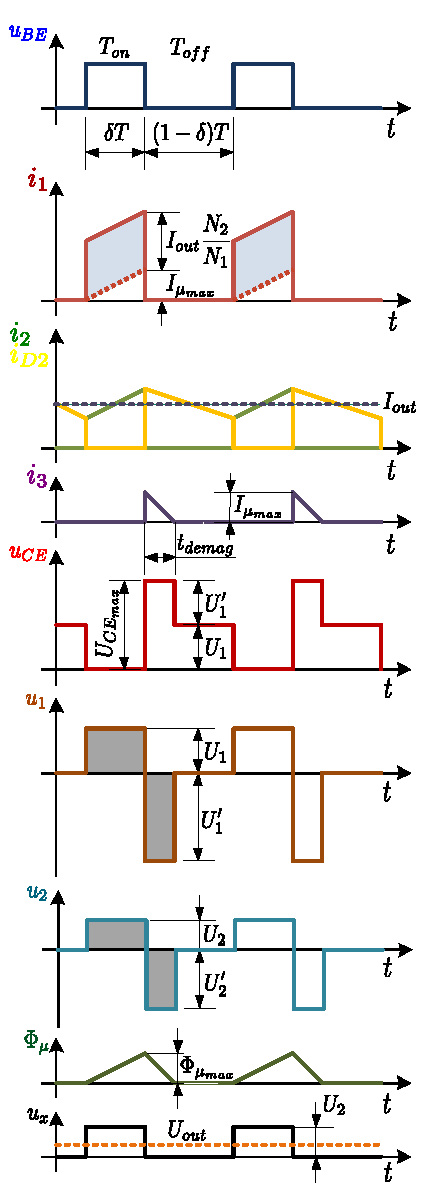
\includegraphics[width=0.7\linewidth]{Forward_converter_wave.pdf}
      \caption{Průběhy veličin propustného měniče s akumulační tlumivkou a demagnetizačním 
      vinutím}
      \label{enz:fig_Forward_demag_wave} 
    \end{figure}                          
    
    \begin{equation}\label{ENZ:eq_forward_u1_demag}
     U_1'=u_3\frac{N_1}{N_3} = U_1\frac{N_1}{N_3}
    \end{equation}
    Tento stav, kdy  $u_1 = -U_1$ a  $u_3 = U_1$, trvá po dobu, než tok $\Phi_\mu(t)$ klesne z 
    počáteční hodnoty $\Phi_{\mu_{max}}$ na nulu. K tomu je třeba konečné doby $t_{demag}$, neboť 
    $U_1$ není nekonečné a proto strmost poklesu $\frac{d\Phi}{dt}$ nemůže být nekonečně velká. 
    Velikost $U_1$ je v této době konstantní a proto klesá tok lineárně. Celý jev se nazývá 
    \emph{demagnetizací jádra}.
    
    Během demagnetizace se předává magnetizační energie jádra zpět do zdroje pomocí proudu 
    $i_3(t)$. Proud $i_3(t)$ je přímo úměrný klesajícímu toku $\Phi_\mu(t)$ takto:
    \begin{equation}\label{ENZ:eq_imag_phi_forward}
     i_3(t) = \frac{1}{L_3}\int{u_3}dt = \frac{1}{L_3}\int{\frac{N_3d\Phi_\mu(t)}{dt}}dt =
     \frac{N_3\Phi_\mu(t)}{L_3}
    \end{equation}
    Po skončení demagnetizace (uplynutí $t_{demag}$) je již magnetický tok nulový, jádro je 
    energeticky neutrální, proto i napětí $u_1$, $u_2$, $u_3$ skokem zanikají na nulu. V 
    neutrálním stavu soustava setrvává až do skončení doby $(1-\delta)T$, tj. do zapnutí 
    tranzistoru.
    
    Pro magnetický tok během procesu demagnetizace musí platit:
    \begin{equation}\label{ENZ:eq_phi_mag_forward}
     \Phi_\mu(t) = \Phi_{\mu_{max}} - \frac{\int{u_1(t)dt}}{N_1} = \Phi_{\mu_{max}} -
     \frac{U_1't}{N_1}
    \end{equation}
    Po uplynutí $t_{demag}$ je tok nulový. Položíme-li tedy $\Phi_\mu(t)$ dle
    (\ref{ENZ:eq_phi_mag_forward}) rovný nule, lze odsud vyjádřit $t_{demag}$.
    \begin{equation}\label{ENZ:eq_tdemag_forward}
     t_{demag} = \frac{N_1\Phi_{\mu_{max}}}{U_1'}
    \end{equation}
    Za $\Phi_{\mu_{max}}$ dosadíme vztah (\ref{ENZ:eq_forward_phi_max}) a za $U_1$  vztah
    (\ref{ENZ:eq_forward_u1_demag}). Tím dostaneme:
    \begin{equation}\label{ENZ:eq_tdemag_N1N3_forward}
     t_{demag} = \frac{N_3}{N_1}\delta T
    \end{equation}
    Je zřejmé, že musíme zajistit, aby $(1-\delta)T > t_{demag}$, jinak by tok ještě nestačil
    úplně zaniknout a už bychom znovu spínali tranzistor. V průběhu dalšího sepnutí by se tok (a
    magnetizační proud) zvýšil opět o hodnotu $\Phi_{\mu_{max}}$ (resp.  $I_{\mu_{max}}$, ale už z
    nenulové počáteční hodnoty a tak by neustále vzrůstal (během dalších period by se
    „naintegroval“ teoreticky na hodnotu $\rightarrow\infty$), až by došlo k přesycení jádra a tím
    k prudkému lavinovitému růstu magnetizačního proudu (neboť by současné klesla indukčnost
    $L_1$). Jev by postupoval až do zničení tranzistoru. Z výše uvedeného důvodu musí být
    maximální střída $\delta$ omezena na hodnotu:
    \begin{equation}\label{ENZ:eq_forward_delta_max}
    \delta_{max} = \frac{t_{on}}{t_{on}+t_{demag}}
    \end{equation}
    Dosazením (\ref{ENZ:eq_tdemag_N1N3_forward}) za $t_{demag}$ dostaneme:
    \begin{equation}\label{ENZ:eq_forward_delta_max1}
    \delta_{max} = \frac{N_1}{N_1+N_3}
    \end{equation}
    Výstupní napětí $U_{out}$ je rovno \emph{střední hodnotě napětí} $u_X$ a platí proto:
    \begin{equation}\label{ENZ:eq_uout_forward_delta}
    U_{out} = U_1\frac{N_2}{N_1}\frac{t_{on}}{t_{on} + t_{off}} = U_1\frac{N_2}{N_1}\delta
    \end{equation}
    
   %---------- Proudové a napěťové dimenzování součástek -----------------------------------------
  \subsection{Proudové a napěťové dimenzování součástek}
    V době $t_{demag}$ je tranzistor namáhán napětím $U_{{CE}_{max}}$:
    \begin{equation}\label{ENZ:eq_dim_Ucemax}
      U_{{CE}_{max}} = U_1 + U_1' = U_1 + \frac{N_3}{N_1}U_1 = U_1\frac{N_1+N_3}{N_1}
    \end{equation}
    \begin{itemize}[noitemsep]
     \item Volíme-li $N_3 < N_1$, je $U_1' > U_1$ a tedy namáhání $U_{{CE}_{max}} > 2U_1$. Zato
           je ale maximální dovolená střída $\delta_{max} > 0,5$ a je tedy větší maximální
           dosažitelné výstupní napětí.
     \item Volíme-li $N_3 > N_1$, je $U_1' < U_1$ a je tedy  $U_1 < U_{{CE}_{max}} < 2U_1$. Zato
           je ale maximální dovolená střída $\delta_{max} < 0,5$ a je tedy menší maximální
           dosažitelné výstupní napětí.
    \end{itemize}
    Volba  poměru  $N_3/N_1$ proto záleží na tom, co je v dané aplikaci více kritické, zda
    napěťové namáhání tranzistoru,  či co největší dosažitelné výstupní napětí (s neměnným
    převodem  $N_2/N_1$). V praxi se nejčastěji volí $N_3 = N_1$ z důvodů snadného souběžného
    (\emph{bifilárního}) vinutí obou cívek - viz později.
    
    \begin{itemize}
      \item \emph{Proudové a dimenzování $T_1$:}
         \newline Zanedbáme-li magnetizační proud, pak lze psát, viz. obr.
         \ref{enz:fig_Forward_demag_wave}, pro špičkovou, střední a efektivní hodnotu
         kolektorového proudu tranzistoru následující rovnice:
          \begin{align}
              I_{1_{max}} &= I_{out}\frac{N_2}{N_1}             \\
              I_{1_{av}}  &= I_{out}\frac{N_2}{N_1}\delta       \\
              I_{1_{rms}} &= I_{out}\frac{N_2}{N_1}\sqrt{\delta}
          \end{align}
      \item \emph{Proudové a napěťové dimenzování $D_1$:}
          \begin{align}
              I_{D_{1max}} &= I_{out}                \\
              I_{D_{1av}}  &= I_{out}\delta          \\
              I_{D_{1rms}} &= I_{out}\sqrt{\delta}   \\
              U_{D_{1Rmax}}&= U_1\frac{N_2}{N_3}
          \end{align}
      \item \emph{Proudové a napěťové dimenzování $D_2$:}
          \begin{align}
              I_{D_{2max}} &= I_{out}                \\
              I_{D_{2av}}  &= I_{out}(1-\delta)      \\
              I_{D_{2rms}} &= I_{out}\sqrt{1-\delta} \\
              U_{D_{2Rmax}}&= U_1\frac{N_2}{N_1}
          \end{align}
      \item \emph{Proudové a napěťové dimenzování $D_3$:}
          \begin{align}
              I_{D_{3max}} &= I_3        = I_{\mu_{max}}\frac{N_1}{N_3}           
                            = \frac{U_1\delta_{max}T}{L_1}\cdot\frac{N_1}{N_3}                \\
              I_{D_{3av}}  &= I_{3_{av}} = \frac{I_3}{2}\delta                                \\
              I_{D_{3rms}} &=  \sqrt{\frac{1}{T}\int_0^{t_{demag}}
                              {\left(I_3\frac{t}{t_{demag}}\right)^2}dt}            \nonumber \\ 
                           &= \frac{I_3}{\sqrt{3}}\sqrt{\frac{t_{demag}}{T}}                  \\
              U_{D_{3Rmax}}&= U_1 + U_1\frac{N_3}{N_1}
          \end{align}
    \end{itemize}
    \begin{tcnote}
      Všimneme si, že funkce tohoto měniče je kromě transformátoru zcela analogická funkci
      snižujícího měniče z kap. \ref{aes:sec002}. Horní spínač je zde rozdělen tak, že tranzistor je
      na primární straně (pro větší podobnost s obr. \ref{enz:fig_003} lze v obr.
      \ref{aes:fig074} vzájemně zaměnit umístění tranzistoru a primárního vinutí
      transformátoru, tj. z kladného pólu $U_{in}$ nejprve tranzistor). Dioda $D_2$, tvořící s
      tranzistorem horní spínač, je až na sekundární straně. Dioda $D_1$ jen odděluje výstupní obvod
      od sekundárního napětí v době, kdy je záporné, protože  toto napětí nemůže mít nenulovou
      stejnosměrnou složku (stejně tak ani napětí $u_1$ a $u_3$).
    \end{tcnote}

  \subsection{Přehled metod demagnetizace jádra transformátoru}

    \luagraphic[0.8]{aes_fig073.pdf}{Transformátor jednočinného propustného měniče pracuje v prvním
    kvadrantu hysterezní smyčky}{aes:fig073}

    V kapitole \ref{ENZ:kap_forward_converter_describe} byl popsán jeden z možných způsobů, jak
    demagnetizovat jádro transformátoru, tak aby v dalším pracovním cyklu nedošlo k posunu
    pracovního bodu magnetického materiálu jádra a následně k jeho přesycení. Velikost
    magnetizačního proudu je dle vztahu \ref{ENZ:eq_forward_imag_max} dána poměrem napěťové plochy
    $U_{in}\cdot t_{on}$ přiložené na vinutí primární cívky a hodnotou její magnetizační indukčnosti
    ($L_{mag} = L_{1}$) 
    \begin{equation}
       i_{mag} = \frac{U_{prim}\cdot{t_{on}}}{L_{mag}}.
    \end{equation}
    
    Pracovní oblast transformátoru je v prvním kvadrantu, jak naznačuje obr. \ref{aes:fig073}, neboť
    polovodičový spínač přikládá mezi svorky primárního vinutí pouze unipolární pulzy. Měnič se také
    proto nazývá \emph{jednočinný}, protože energie je ze zdroje předávána do zátěže pouze jedenkrát
    za periodu, v jednom tzv. aktivním běhu, tj. v době $t_{on}$, kdy je tranzistor sepnut a
    magnetická indukce se v jádře zvyšuje z hodnoty remanentní indukce $B_r$ o velikost magnetického
    zdvihu $\Delta B$.
    
    \begin{figure}[ht!]
    \centering
    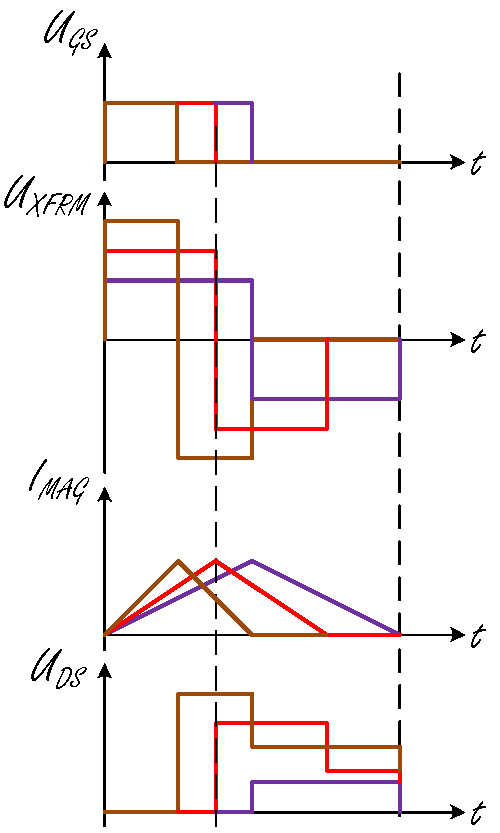
\includegraphics[width=0.5\linewidth]{imag_forward_converter.pdf}
    \caption[Magnetizační proud]{Vrcholová hodnota magnetizačního proudu je konstantní pro
             jakékoliv velikosti vstupního napětí, neboť regulační smyčka zajistí, aby napěťová
             plocha $V_{in}\cdot t_{on}$ byla konstantní}
    \label{enz:fig_imag_forward_converter}
    \end{figure}
    
    Pokud bychom měřili magnetizační proud primárního vinutí, dospěli bychom k průběhům na obr.
    \ref{enz:fig_imag_forward_converter}, jenž vykazují stejnou vrcholovou hodnotu pro různé hodnoty
    vstupního napětí. Je to dáno tím, že pokud měnič během měření pracoval v uzavřené regulační
    smyčce, bude součin $V_{in}\cdot t_{on}$ konstantní a za předpokladu, že magnetizační indukčnost
    je též neměnná, pak dle předchozí rovnice dospějeme $i_{mag_{max}} = konst$.
   
    %------------- Jednočinný propustný měnič s aktivním clampingem ------------------------------
  \subsection{Jednočinný propustný měnič s aktivním clampingem}\label{ENZ:kap_afwdconv}  
    Obecně pro všechny varianty  propustných měničů s transformátorem lze říci, že jsou vhodné pro
    přenos velkých výkonu. Je to dáno principem činnosti, kdy proud podílející se na přenosu výkonu
    se nepodílí na magnetizaci jádra transformátoru (teče v době $t_{on}$ a to jak na sekundární
    straně tak i na primární - kompenzace magnetických účinku). Může se proto zvyšovat, aniž by
    rostlo sycení jádra transformátoru. Toto sycení je určeno pouze integrálem primárního napětí a
    počtem primárních závitu. Lze proto zvýšením pracovního kmitočtu docílit zmenšení velikosti
    transformátoru, jak to bylo vysvětleno na konci kap. \ref{ES:kap_simple_rozbor_trafa}.
    \begin{figure}[ht!]
      \centering
      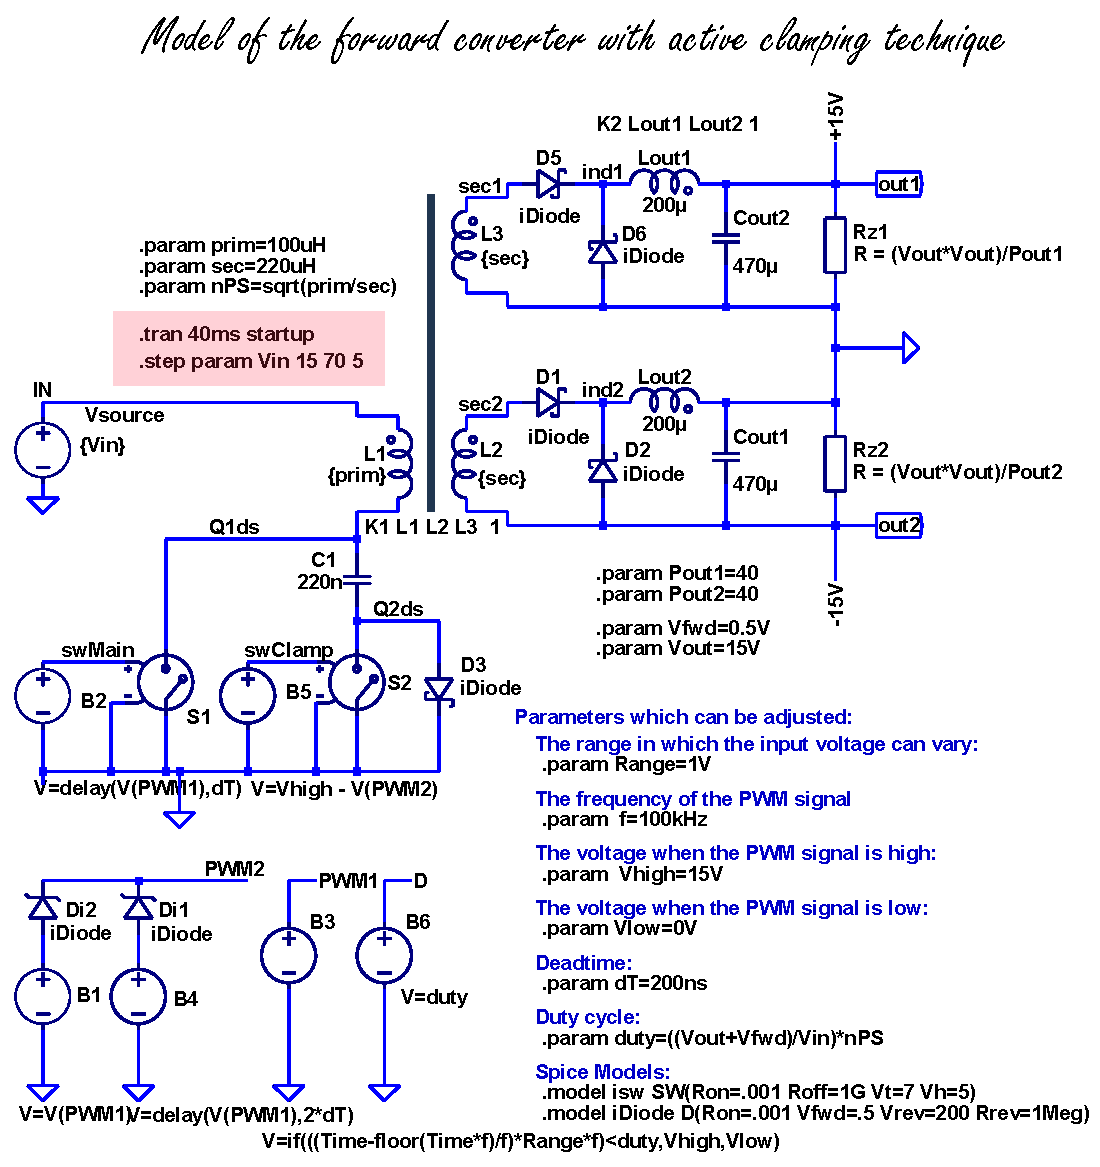
\includegraphics[width=\linewidth]{forward_converter_active_ltspice_model.pdf}
      \caption[Propustný měnič s aktivním clampingem]{Propustný měnič s aktivním clampingem}
      \label{enz:fig_imag_a_lt_frwd_conv}
    \end{figure}   



    %-----------------------------------------------------------------------------------------------

   %------------- Jednočinný blokující měnič -------------------------------------------------------
    % !TeX spellcheck = cs_CZ
\section{Jednočinný blokující měnič}\label{ENZ:ssec_01}\hypertarget{ENZ:ssec_01}
  Základem tohoto měniče je „invertující měnič se společnou tlumivkou“ z kapitoly \ref{aes:sec003}. 
  Všimneme si, že z původního schématu (obr. \ref{enz:fig_007a}) vymizela tlumivka, jejíž funkci 
  nyní zastane transformátor. 
  \begin{figure}[ht!]
    \centering
    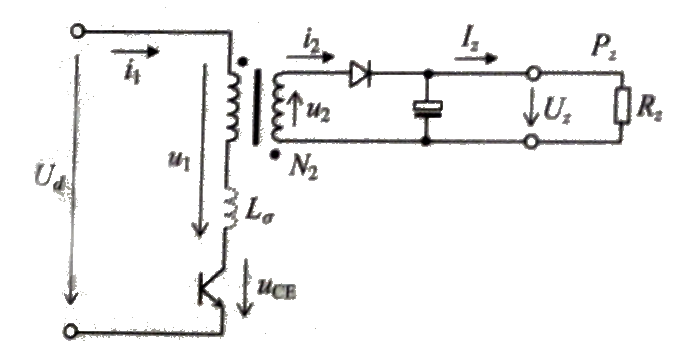
\includegraphics[width=0.6\linewidth]{flyback_sch.png}
    \caption{Základní zapojení jednočinného blokujícího měniče.}
    \label{enz:fig_008}
  \end{figure} 
  Princip činnosti je vlastně úplně stejný, pokud si uvědomíme, že jádro nynějšího transformátoru 
  je magnetováno stejně jako jádro tlumivky na obr. \ref{enz:fig_007a}, viz. průběh $i_L(t)$ v 
  obr. \ref{enz:fig_007b} a průběh $\Phi_\mu(t)$ v obr.\ref{enz:fig_008}. Jediný rozdíl je v tom, 
  že stejných magnetických poměrů je nyní dosaženo pomocí dvou vinutí místo původního jednoho (v 
  době $t_1$ pomocí $L_1$ a v době $t_2$ pomocí $L_2$). Tím se dosáhne galvanického oddělení. 
  Vznikl tak transformátor, ovšem režim jeho činnosti je takový, že magnetické účinky v jádře se 
  podobají tlumivce. Režim je zcela odlišný od režimu transformátoru v propustných měničích.
 
  \begin{figure}[ht!]
    \centering
    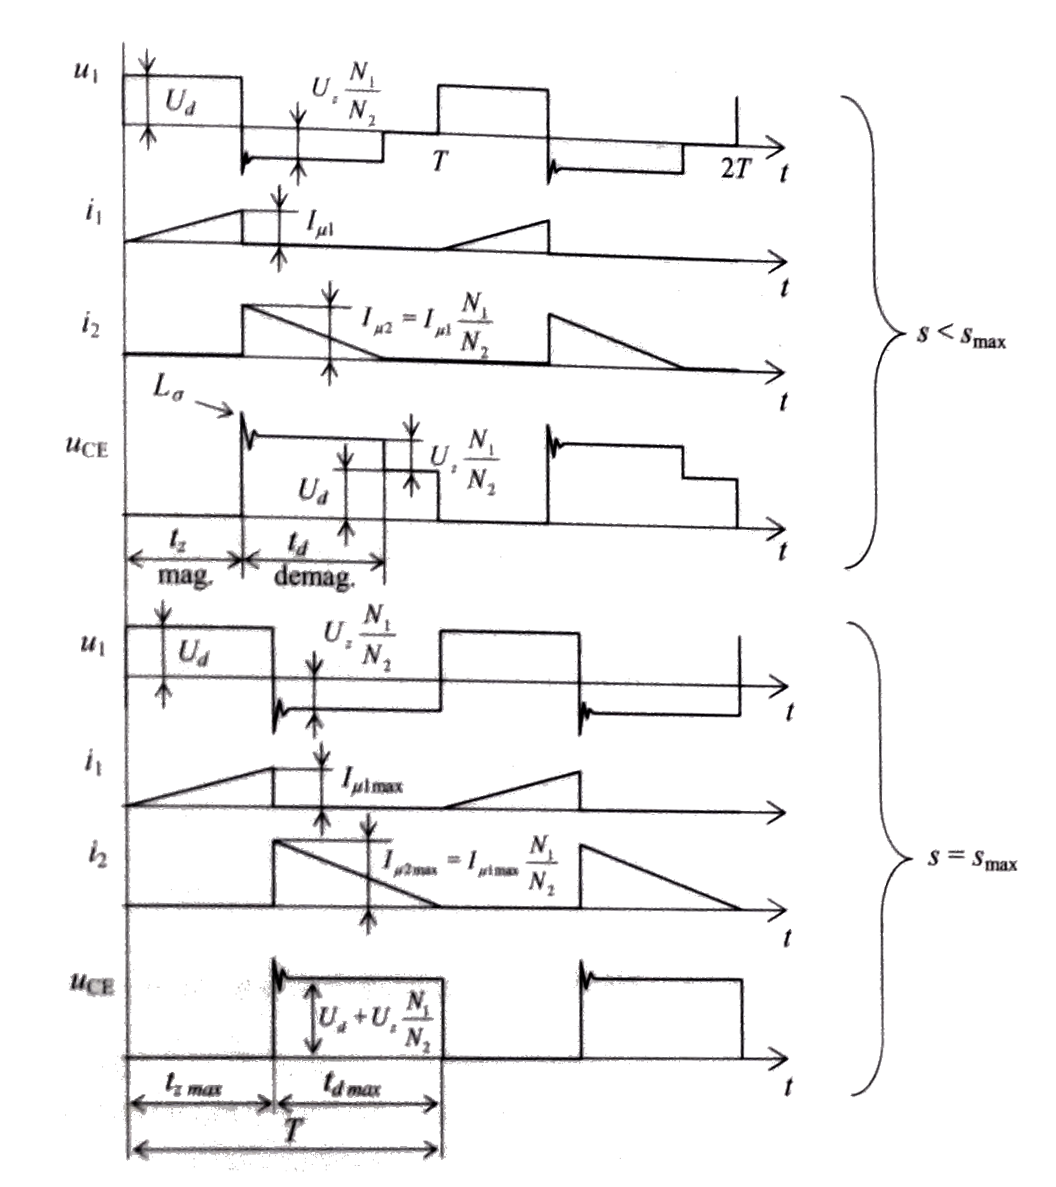
\includegraphics[width=\linewidth]{flyback_wave.png}
    \caption{Časové průběhy všech důležitých veličin v blokujícím měniči.}
    \label{enz:fig_009}
  \end{figure} 
  Indukčnost \(L_\sigma\) představuje \emph{parazitní rozptylovou indukčnost transformátoru}. 
  Rozptylová indukčnost je nežádoucí, protože způsobuje přídavný napěťový překmit na tranzistoru 
  v okamžiku vypínání. Velikost překmitu roste s velikostí proudu, tedy s velikostí přenášeného 
  výkonu. To je značná nevýhoda blokujících měničů.
  
  Činnost měniče vyplývá z časových průběhů na obr. \ref{enz:fig_009}. V horní části jsou 
  nakresleny průběhy při menší střídě \(\delta\), v dolní jsou tytéž průběhy, ale při maximální 
  střídě. V časovém intervalu \(t_z\) je tranzistor sepnut, tudíž probíhá \emph{magnetizace} 
  transformátoru proudem \(i_1\) pomocí \emph{primárního} vinuti. Dioda sekundárního usměrňovače 
  je v té době zavřena, zátěž je odpojena od transformátoru a napájena pouze z nabitého 
  kondenzátoru. V intervalu \(t_d\) je tranzistor vypnut, tudíž probíhá \emph{demagnetizace} 
  transformátoru pomocí \emph{sekundárního} vinutí. Dioda je v té době otevřena a kondenzátor je 
  napájen demagnetizačním trojúhelníkovým proudovým pulsem \(i_2\). V té chvílí je sekundární 
  vinutí přes diodu připojeno na \emph{konstantní} napětí \(U_z\) kondenzátoru a tímto napětím je 
  demagnetováno. Aby bylo napětí konstantní, kondenzátor musí mít dostatečně velkou kapacitu. 
  Magnetizační proud \(i_1\), roste \emph{lineárně} s časem, protože je integrálem z 
  \emph{konstantního} napětí \(+U_d\). Podobně demagnetizační proud \(i_2\) klesá \emph{lineárně} 
  s časem, protože je integrálem z \emph{konstantního} napětí \(-U_z\). V dolní části obr. 
  \ref{enz:fig_009} jsou nakresleny průběhy při maximální střídě \(\delta_{max}\). Je to mezní 
  stav, při kterém je demagnetizace dokončena přesně na konci pracovní periody \(T\) a 
  magnetizační tok právě zaniká. Teoreticky je možné střídu zvětšit, pak nedojde k úplné 
  demagnetizaci a transformátor začne pracovat v režimu \emph{nepřerušovaného} spojitého 
  magnetického toku, viz horní průběh na obr. \ref{enz:fig_010}. V tom případě bude sice 
  přenášený výkon větší, ovšem za cenu, že režim je \emph{neoptimální}. Důvod spočívá v tom, že 
  minimální tok \(\Psi_{min}\) sice vzroste, ale maximální zdvih pilovitého zvlnění 
  \(\Delta\Psi\) se zvětšit nemůže a zůstává \emph{konstantní}. Energie \(\Delta W\), přenesená v 
  jednom pracovním cyklu, je dána rovnicí
  \begin{align}
    \Delta W 
      &= \frac{1}{2}\frac{\Psi_{max}^2}{L_1} 
       - \frac{1}{2}\frac{\Psi_{min}^2}{L_1}   
       = \frac{1}{2}\frac{(\Psi_{min}+\Delta\Psi)^2}{L_1} 
       - \frac{1}{2}\frac{\Psi_{min}^2}{L_1}   \nonumber \\
      &= \frac{1}{2L_1}\left(2\Psi_{min}\Delta\Psi+\Delta\Psi^2\right) \label{ENZ:eq_001}
  \end{align}
  
  \begin{figure}[ht!]
    \centering
    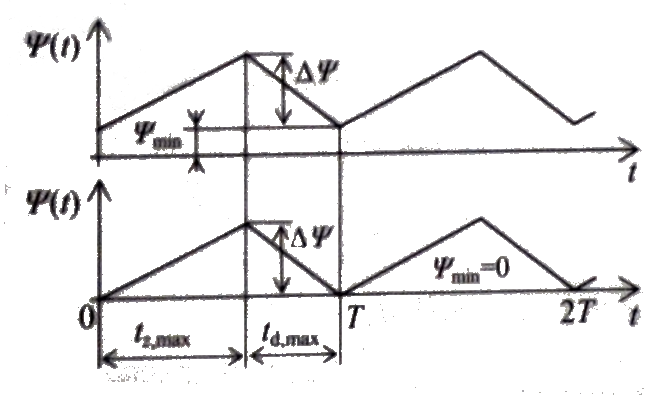
\includegraphics[width=0.6\linewidth]{flyback_tok.png}
    \caption{Spřažený tok transformátoru při podmínce \(\Psi_{min}>0\) a \(\Psi_{min}=0\)}
    \label{enz:fig_010}
  \end{figure} 
  
  Vidíme, že množství přenášené energie \(\Delta W\) je dáno \emph{druhou} mocninou zdvihu 
  \(\Delta\Psi\), ale pouze \emph{první} mocninou minimální hodnoty \(\Psi_{min}\). Růst hodnoty 
  \(\Psi_{min}\) je proto energeticky málo účinný a tudíž nevýhodný. Optimální stav nastává při 
  podmínce \(\Psi_{min} = 0\). Měnič bude analyzován a navrhován právě při dodržení této podmínky.
  \begin{align}
    \shortintertext{Pracovní střídaje definována rovnici}
    \delta       &= \frac{t_z}{T}. \label{ENZ:eq_002} \\
    \shortintertext{Pro maximální střídu zřejmé platí vztah}
    \delta_{max} &= \frac{t_{z_{max}}}{t_{z_{max}}+t_{d_{max}}}
                  = \dfrac{1}{1+\dfrac{t_{d_{max}}}{t_{z_{max}}}}. \label{ENZ:eq_003} \\
    \shortintertext{V době zapnutí poroste magnetizaění proud \(i_1\) se strmostí}
    \der{i_1}{t} &= \frac{I_{{\mu1}_{max}}}{t_{z_{max}}} 
                  = \frac{U_d}{L_1}  \label{ENZ:eq_004} \\
    \shortintertext{V době vypnutí bude magnetizaění proud \(i_2\) klesat (v absolutní hodnotě) 
                    se strmostí}
    \der{i_2}{t} &= \frac{I_{{\mu2}_{max}}}{t_{d_{max}}} 
                  = \frac{U_z}{L_2}  \label{ENZ:eq_005}
  \end{align}    
  Z rovnic (\ref{ENZ:eq_005}) a (\ref{ENZ:eq_004}) plyne pomocná rovnice
  \begin{align}
    \frac{t_{d_{max}}}{t_{z_{max}}} 
      &= \frac{U_d L_2 I_{{\mu2}_{max}}}{U_z L_1 I_{{\mu1}_{max}}} \label{ENZ:eq_006} \\
    \shortintertext{Má-li transformátor těsnou vazbu \(k \rightarrow 1\), zřejmě platí}  
    \frac{L_2}{L_1} = \frac{N_2^2}{N_1^2} \label{ENZ:eq_007} \\
    \shortintertext{Z proudového převodu transformátoru plyne}
    \frac{I_{{\mu2}_{max}}}{I_{{\mu1}_{max}}}
      &= \frac{N_1}{N_2}. \label{ENZ:eq_008} \\
    \shortintertext{Po dosazení rovnic (\ref{ENZ:eq_008}) a (\ref{ENZ:eq_007}) do
                   (\ref{ENZ:eq_006}) získáme vztah}
    \frac{t_{d_{max}}}{t_{z_{max}}} 
      &= \frac{U_d N_2}{U_z N_1}  \label{ENZ:eq_009} \\
    \shortintertext{Rovnici (\ref{ENZ:eq_009}) dosadíme do (\ref{ENZ:eq_003}). Tak získáme výraz 
                    pro maximální střídu:}
    \delta_{max} 
      &= \dfrac{1}{1+\dfrac{U_d N_2}{U_z N_1}}. \label{ENZ:eq_010} 
  \end{align}
  V době demagnetizace se sekundární demagnetizační napětí \(U_z\) přetransformuje s převodem na 
  primár a zde se přičte k mezilehlému napětí \(U_d\). Tranzistor je namáhán součtem těchto 
  napětí:
  \begin{align}
    U_{CE_{max}} &= U_d + U_z\frac{N_1}{N_2}   \qquad \Rightarrow \qquad 
    U_z\frac{N_1}{N_2} = U_{CE_{max}} - U_d    \label{ENZ:eq_011} \\
    \shortintertext{Rovnici (\ref{ENZ:eq_011}) dosadíme do (\ref{ENZ:eq_010}). Pak bude mít 
                    maximální střída velikost}
    \delta_{max} &= 1-\frac{U_d}{U_{CE_{max}}} \label{ENZ:eq_030}
  \end{align}
  Napětí \(U_d\) je zadáno. Maximální pracovní napětí tranzistoru \(U_{CE_{max}}\) je nutno 
  zvolit s ohledem na bezpečný provoz. Z rovnice (\ref{ENZ:eq_011}) plyne, že musí být bohužel 
  vždy splněna nerovnost
  \begin{equation}\label{ENZ:eq_012}
   U_{CE_{max}} > U_d,
  \end{equation}
  jinak nemůže měnič vůbec pracovat. Na hladině \(U_d = \qty{350}{V}\) se volí nejvýše 
  \(U_{CE_{max}} =  2\cdot U_d\) potom vychází \(\delta_{max} = 0,5\). Na hladině \(U_d = 
  \qty{600}{V}\) se musí volit poměr daleko menší, např. \(U_{CE_{max}} =  1,1\cdot U_d\) protože 
  běžně lze použít tranzistory MOSFET se závěrným napětím okolo \(\qty{800}{V}\). Ale i tak, 
  vychází maximální střída pouze \(\delta_{max} = 0,09\), což vede k naprosto neoptimálnímu 
  návrhu měniče. Potřebný počet sekundárních závitů plyne z rovnice (\ref{ENZ:eq_011}), případně 
  z rovnice (\ref{ENZ:eq_010}):
  \begin{equation}\label{ENZ:eq_013}
    N_2 = N_1\frac{U_z}{U_{CE_{max}}-U_d}, \qquad 
    N_1 = N_2\frac{U_z}{U_d}\frac{1-\delta_{max}}{\delta_{max}}
  \end{equation}
  
  \subsection{Návrh transformátoru}
    Výkon přenášený transformátorem je nutno určit pomocí magnetizační energie a pracovního 
    kmitočtu. Ze vztahu (\ref{ENZ:eq_002}) vyplývá pomocná rovnice
    \begin{align}
      t_z      &= \delta T = \frac{\delta}{f}.         \label{ENZ:eq_014} \\ 
      \shortintertext{Ze vztahu (\ref{ENZ:eq_004}) plyne další pomocná rovnice} 
      I_{\mu1} &= \frac{U_d t_z}{L_1}.                 \label{ENZ:eq_015} \\ 
      \shortintertext{Energie, načerpaná v době sepnutí primárním vinutím a bezeztrátově 
                      přenesená v jednom pracovním cyklu do zátěže, má zřejmě velikost}
      W_{L1}   &= \frac{1}{2}L_1I_{\mu1}^2 
                = \frac{1}{2}U_dI_{\mu1}t_z.           \label{ENZ:eq_016} \\
      \shortintertext{Má-li pracovní cyklus periodu \(T\), pak \emph{střední} neboli \emph{činný} 
                      výkon, přenášený do zátěže, bude}
      P_z      &= \frac{W}{T} = \frac{1}{2}U_dI_{\mu1}\frac{t_z}{T} 
                = \frac{1}{2}U_dI_{\mu1}\delta.        \label{ENZ:eq_017} \\
      \shortintertext{Do rovnice (\ref{ENZ:eq_017}) dosadíme (\ref{ENZ:eq_015}). Po úpravě 
                     získáme vztah}
      P_z      &= \frac{U_d^2\delta}{2L_1}t_z
                = \frac{U_d^2\delta}{2L_1}\frac{t_z}{fT}
                = \frac{U_d^2\delta}{2L_1}\frac{\delta}{f}
                = \frac{U_d^2\delta^2}{2fL_1}.          \label{ENZ:eq_018}
    \end{align}
    Potom bude transformátor schopen přenést zvolený maximální výkon\footnote{Blokující měnič 
    nemůže být nad tuto zvolenou hodnotu ani krátkodobě přetěžován - na rozdíl od propustných 
    měničů.} při maximální střídě:
    \begin{align}
      P_{z_{max}} &= \frac{U_d^2\delta_{max}^2}{2fL_1}           \label{ENZ:eq_019} \\ 
      \shortintertext{Tentýž maximální výkon lze též vyjádřit rovnicí (\ref{ENZ:eq_017}):}
      P_{z_{max}} &= \frac{1}{2}U_d I_{{\mu1}_{max}}\delta_{max} \label{ENZ:eq_020} \\
      \shortintertext{Z rovnice (\ref{ENZ:eq_019}) plyne požadovaná velikost primární indukčnosti}
      L_1         &= \frac{U_d^2\delta_{max}^2}{2fP_{z_{max}}}   \label{ENZ:eq_021} \\
      \shortintertext{Z rovnice (\ref{ENZ:eq_020}) plyne maximální velikost primárního 
                      magnetizačního proudu}
      I_{{\mu1}_{max}} &= \frac{2P_{z_{max}}}{U_d\delta_{max}}   \label{ENZ:eq_022} \\
      \shortintertext{Tentýž primární magnetizační proud (trojúhelníkového tvaru) má efektivní 
                      hodnotu}
      I_{{\mu1}_{ef}} &= I_{{\mu1}_{max}}\sqrt{\frac{\delta_{max}}{3}} \label{ENZ:eq_023}
    \end{align}
    Rovnice (\ref{ENZ:eq_021}), (\ref{ENZ:eq_022}) a (\ref{ENZ:eq_023}) jsou pro optimální návrh 
    transformátoru stěžejní. Návrh transformátoru je pak naprosto stejný jako návrh tlumivky 
    na feromagnetickém jádře se vzduchovou mezerou podle kapitoly 12. Tam byly vstupními 
    hodnotami pro návrh rovněž indukčnost \(L_1\) a proud \(I_{max}\), odpovídající indukci 
    \(B_{max}\). Jediný rozdíl je v tom, že v okně jádra transformátoru je nutno pamatovat i na 
    existenci sekundárního vinutí, které zřejmě zabere polovinu plochy okna. Proto je nutno 
    modifikovat původní rovnici (12.2.1-3) pro návrh tlumivky, kterou zde znovu uvedeme:
    \begin{align}
      S_0S_j &= \frac{LI_{max}^2k_z}{k_{p_{Fe}}k_{p_{Cu}}B_{max}\sigma} 
             =  \frac{LI_{max}I_{ef}}{k_{p_{Fe}}k_{p_{Cu}}B_{max}\sigma}. \label{ENZ:eq_024}  \\
      \shortintertext{do tvaru}
      \frac{S_0}{2}S_j 
             &= \frac{L_1I_{{\mu1}_{max}}I_{{\mu1}_{ef}}}{k_{p_{Fe}}k_{p_{Cu}}B_{max}\sigma}
              = \frac{L_1I_{{\mu1}_{max}}^2}{k_{p_{Fe}}k_{p_{Cu}}B_{max}\sigma}
                \sqrt{\frac{\delta_{max}}{3}}.                           \label{ENZ:eq_025}  \\
      \shortintertext{Činitel plnění feritového jádra je roven jedné. Rovnici poté upravíme do 
                      konečné podoby}
      S_0S_j &=2\sqrt{\frac{\delta_{max}}{3}} 
                \frac{L_1I_{{\mu1}_{max}}^2}{k_{p_{Cu}}B_{max}\sigma}
                \qquad [\unit{m^4};\unit{H},\unit{A},\unit{T},\unit{A\per\m^2}].   \label{ENZ:eq_026}  \\
      \shortintertext{Dosadíme-li do této rovnice vztahy (\ref{ENZ:eq_021}) a (\ref{ENZ:eq_022}), 
                      získáme druhou podobu rovnice:}
      S_0S_j &=4\sqrt{\frac{\delta_{max}}{3}} 
                \frac{P_{z_{max}}}{k_{p_{Cu}}fB_{max}\sigma}
                \qquad [\unit{m^4};\unit{W},\unit{Hz},\unit{T},\unit{A\per\m^2}].  \label{ENZ:eq_027}
    \end{align}
    Zdálo by se, že je výhodné volit co nejmenší maximální střídu \(\delta_{max}\). Avšak není to 
    vhodné, protože podle rovnice (\ref{ENZ:eq_022}) pak bude příliš veliký magnetizační proud 
    (proudové namáhání tranzistoru). Z rovnic (\ref{ENZ:eq_021}) a (\ref{ENZ:eq_022}) plyne, že 
    transformátor musí mít \textbf{vzduchovou mezeru}, pokud je navržen \emph{optimálně}. 
    Magnetická energie, načerpaná při zapnutí tranzistoru, se totiž nejsnáze ukládá do vzduchové 
    mezery, nikoli do feromagnetika. Proto lze z 12. kapitoly převzít a modifikovat rovnice 
    (12.1.1-3), (12.1.2-3) pro výpočet závitů a délky vzduchové mezery:
    \begin{align}
      N_1 &= \frac{L_1I_{{\mu1}_{max}}}{B_{max}S_j}          \nonumber          \\
      l_v &= \frac{N_1\mu_0I_{{\mu1}_{max}}}{B_{max}} 
           - \frac{l_{Fe}}{\mu_{r_{Fe}}},                    \label{ENZ:eq_028} \\
      \shortintertext{nebo}
      l_v &= \frac{L_1\mu_0I^2_{{\mu1}_{max}}}{B_{max}S_j} 
             - \frac{l_{Fe}}{\mu_{r_{Fe}}},                  \label{ENZ:eq_029}  
    \end{align}
    Postup při návrhu celého měniče je následující:
    \begin{enumerate}[noitemsep]
      \item Je zadáno \(U_z\), \(P{z_{max}}\) ,\(U_z\)
      \item Volíme \(U_{CE_{max}}\),\(f\), \(B_{max}\).
      \item Podle rovnice (\ref{ENZ:eq_030}) určíme maximální střídu \(\delta_{max}\).
      \item Podle rovnic (\ref{ENZ:eq_021}) a (\ref{ENZ:eq_022}) určíme \(L_1\), 
            \(I_{{\mu1}_{max}}\).
      \item Pomocí rovnice (\ref{ENZ:eq_026}) určíme velikost jádra.
      \item Podle rovnice (\ref{ENZ:eq_028}) určíme počet primárních závitů \(N_1\)
      \item Podle rovnice (\ref{ENZ:eq_029}) určíme délku vzduchové mezery \(l_v\).
      \item Podle rovnice (\ref{ENZ:eq_028}) dopočítáme potřebný počet sekundárních závitů \(N_2\)
    \end{enumerate}
    Tím je základní návrh transformátoru i celého měniče ukončen. Zdůrazněme, že návrh odpovídá 
    podmínce \(\Psi_{min}= 0\), která byla vysvětlena v úvodu.
  
  \subsection{Ochrana tranzistoru proti přepětí}
    Indukčnost \(L_\sigma\) na obr. \ref{enz:fig_009} představuje \textbf{parazitní rozptylovou} 
    indukčnost transformátoru, jejíž magnetický tok bohužel není svázán se sekundárním vinutím. 
    Tato nijak neošetřená indukčnost je zapojena do série s tranzistorem. Proto způsobuje v 
    okamžiku vypínacího děje parazitní napěťový překmit na tranzistoru. Tvar napěťového překmitu 
    je naznačen v časových průbězích kolektorového napětí \(u_{CE}(t)\) na obr. 
    \ref{enz:fig_010}. Vzhledem k tomu, že principiálně nelze realizovat transformátor s 
    činitelem vazby \(k = 1\), rozptylovou indukčnost \(L_\sigma\) není možno zcela odstranit. V 
    okamžiku vypínání je v indukčnosti uložena magnetická energie o velikosti
    \begin{equation}\label{ENZ:eq_031}
      W_\sigma = \frac{1}{2}L_\sigma I_{\mu1_{max}},
    \end{equation}
    \begin{figure}[ht!]
      \centering  
      \subcaptionbox{\label{ENZ:fig_011}}{\luafigure[0.4]{flyback01.png}}
      \subcaptionbox{\label{ENZ:fig_012}}{\luafigure[0.4]{flyback02.png}}
      \caption{Možnosti potlačení přepětí způsobeného rozptylovou indukčností transformátoru.}
    \end{figure}
    V zapojení podle obr. \ref{ENZ:fig_011} je vhodné vyladit hodnoty prvků \(R\), \(C\) 
    experimentálně 
    pomocí osciloskopu tak, aby byl kmitavý obvod \(R\), \(C\), \(L_\sigma\) tlumen přibližně 
    kriticky. Na odporu \(R\) se v každém případě ztrácí výkon
    \begin{equation}\label{ENZ:eq_032}
      P_R = 2fW_C = 2f\frac{1}{2}C(2U_d)^2 = 4fCU_d^2,
    \end{equation}
    protože během jednoho pracovního cyklu se kondenzátor přes odpor jednou nabije a jednou 
    vybije. Výkon \(P_R\) může dosahovat relativně velkých hodnot. Z energetického pohledu je 
    výhodnější zapojení podle obr. \ref{ENZ:fig_012}, kde transil musí být dimenzován na výkon
    \begin{equation}\label{ENZ:eq_033}
      P_{trans} = fW_\sigma = \frac{1}{2}L_\sigma I_{\mu1_{max}}^2,
    \end{equation}
    protože během jednoho pracovního cyklu zachycuje pouze energii \(W_\sigma\), což bývá méně 
    než \(2CU_d^2\). Další možností je zapojení podle obr \ref{ENZ:fig_013}. Zde probíhá omezení 
    přepětí na tranzistorech \emph{bezeztrátově}. Činnost měniče zůstává úplně stejná jako v 
    základním zapojení.
    \begin{equation}
      \delta_{max} = 1-\frac{U_d}{U_{CE_{max}}}
    \end{equation}
    \begin{figure}[ht!]
      \centering
      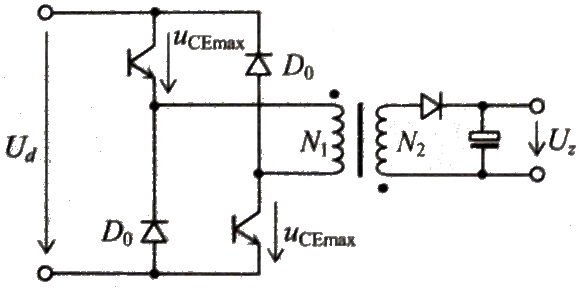
\includegraphics[width=0.7\linewidth]{flyback_2T.png}
      \caption{Přepětí způsobené rozptylovou indukčností transformátoru je potlačeno použitím 
               dvou tranzistorů se záchytnými diodami \(D_0\).}
      \label{ENZ:fig_013}
    \end{figure} 
    Jedná se o dva spínače zapojené do série a spínané současné, jako by se jednalo o spínač 
    jediný. Záchytné diody \(D_0\) slouží pouze k omezení přepětí na tranzistorech, tj. k 
    bezeztrátovému odvedení energie \(W_\sigma\) do ss. meziobvodu. Diody nesmí ovlivňovat 
    činnost měniče. To ovšem znamená, že na jednom tranzistoru musí být ve vypnutém stavu napětí 
    \(U_{CE_{max}}\leqq U_d\), tedy na dvou tranzistorech zapojených v sérii musí být 
    \(2U_{CE_{max}}\leqq 2U_d\). Z rovnice (\ref{ENZ:eq_030}) plyne, že maximální střída musí být 
    omezena na hodnotu
    \begin{align}\label{ENZ:eq_034}
      \delta_{max} &= 1-\frac{U_d}{U_{CE_{max}}} \qquad \rightarrow   \nonumber \\
      \delta_{max} &= 1-\frac{U_d}{2U_{CE_{max}}} = 1 - \frac{U_d}{2U_d} = \frac{1}{2}.
    \end{align}
    Pro případ \(\delta > 0,5\) je zapojení nepoužitelné, protože pak by na každém z tranzistorů 
    muselo být napětí \(U_{CE} > U_d\), což diody \(D_0\) nedovolí.  

   %------------------------------------------------------------------------------------------------

  % ----------------- Metody regulace spínaných zdrojů ---------------------------------------------
  \section{Metody regulace spínaných zdrojů}\label{aes:sec008}
    \subsection{Porovnání regulátoru s napěťovým a proudovým řízením}
      \begin{figure}[ht!]
        \centering
        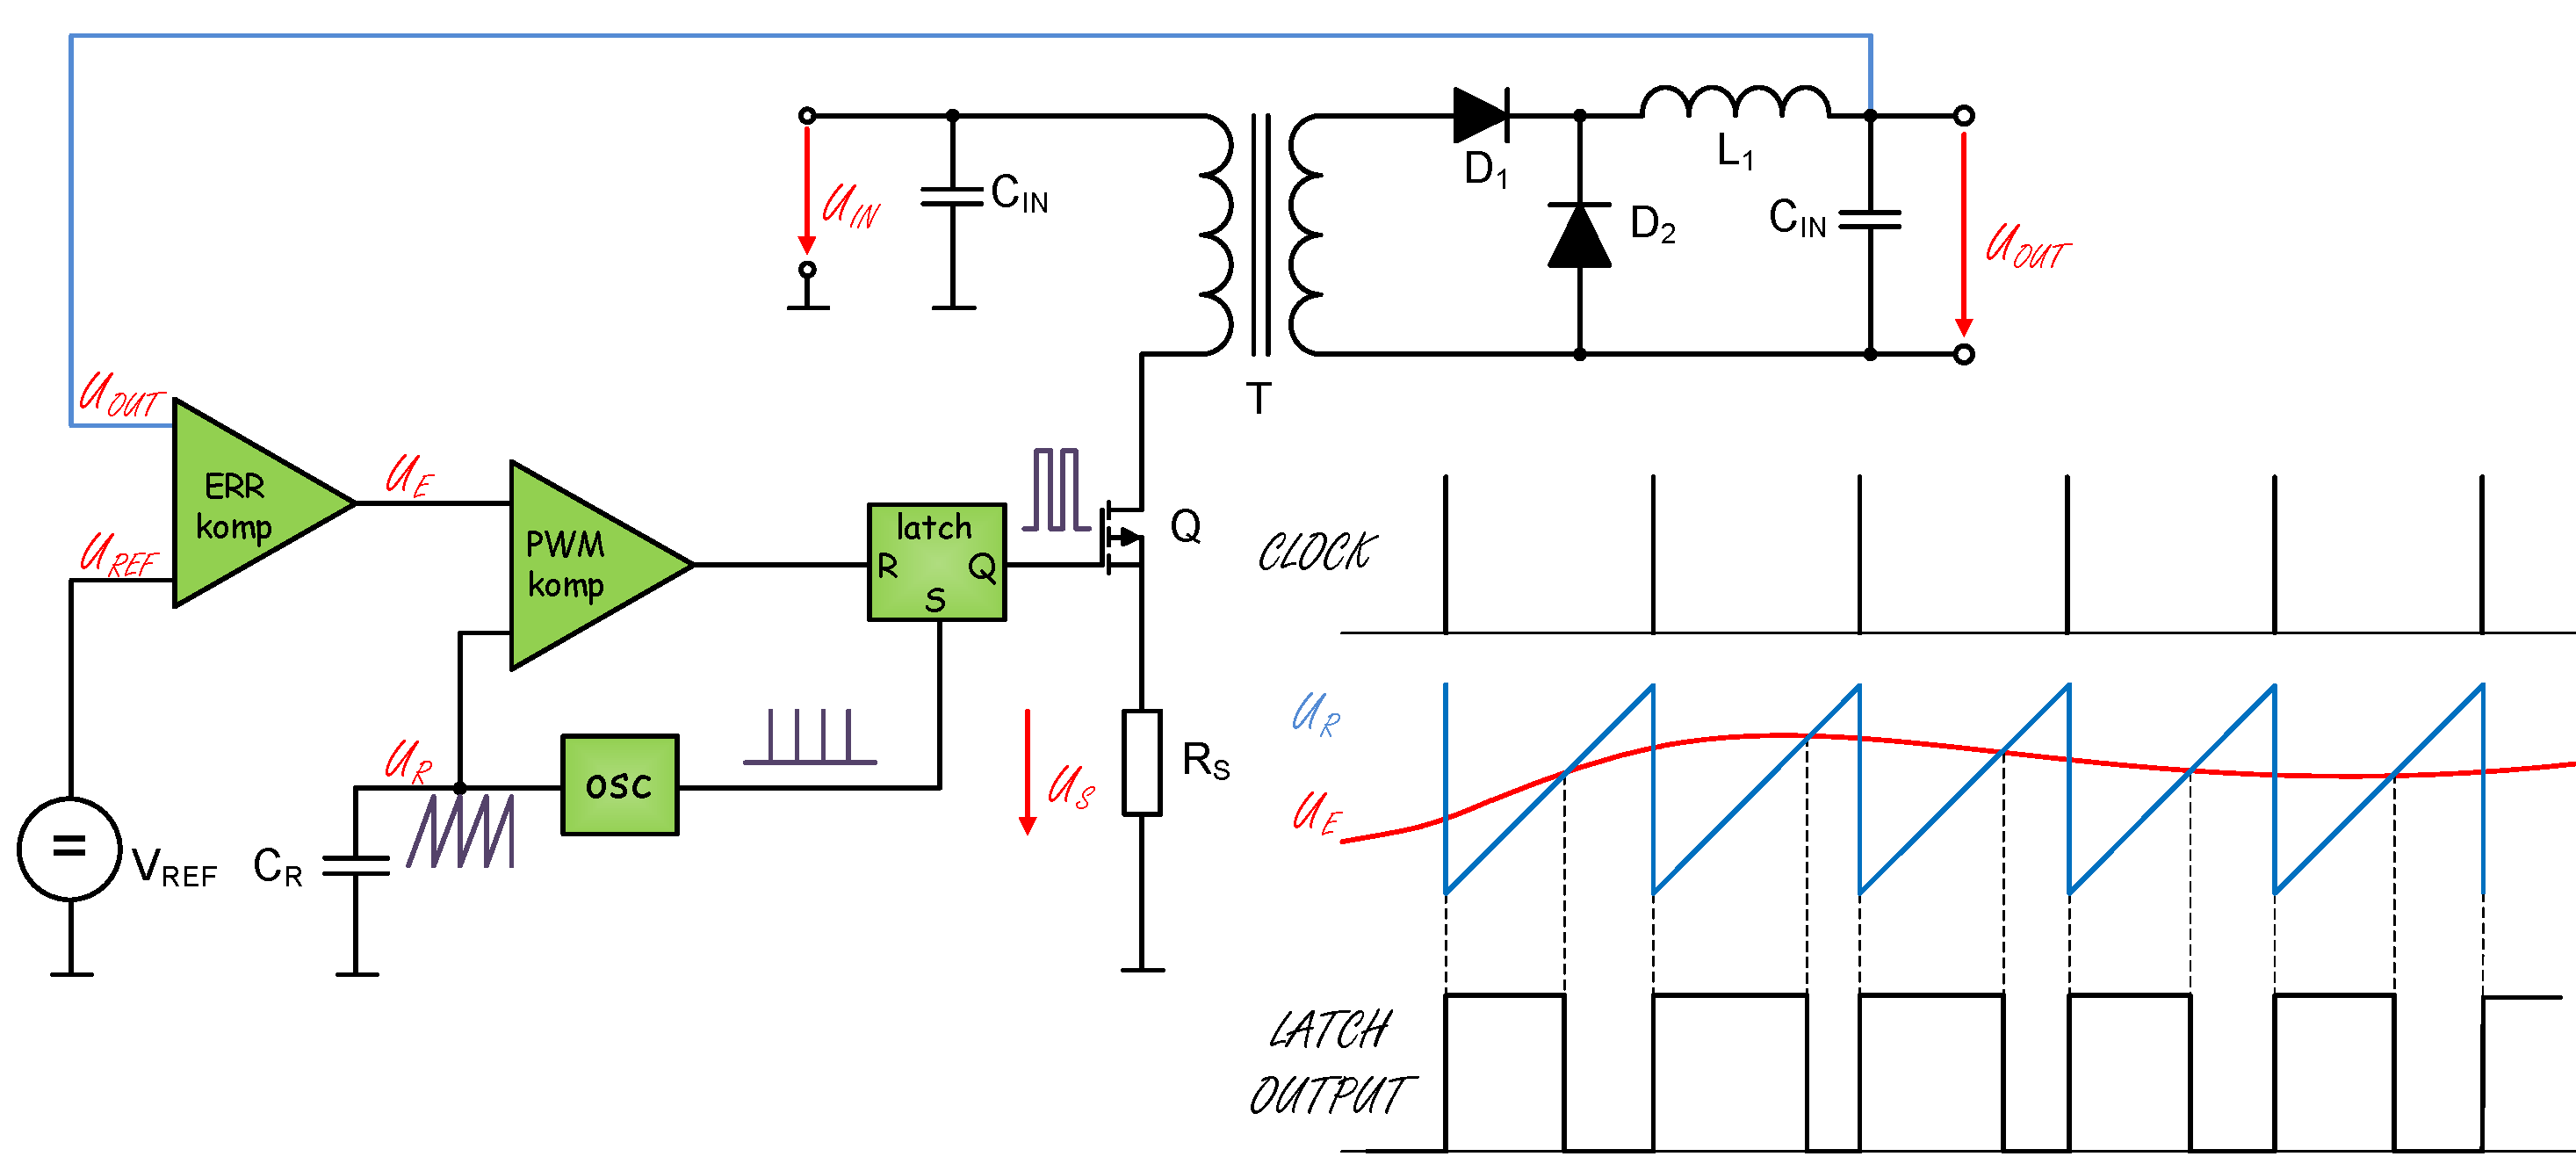
\includegraphics[width=0.9\linewidth]{unitrode_voltage_mode_control.pdf}
        \caption[Regulátor s napěťovým řízením]{Regulátor s napěťovým řízením - Voltage mode
                 control [\cite{SLUA119}]}
        \label{ENZ:fig_V_mode_cntrl}
      \end{figure}
  
  %     The current mode control method uses two control loops --an inner, current control loop
  %     and an outer loop for voltage control. Figure  1 shows a forward converter (buck family)
  %     using current mode control. When the switching transistor is on, current through Rsense is
  %     proportional to the upward ramping filter inductor current. When the ramp voltage Vs
  %     reaches Ve (the amplified  output  voltage  error), the switching transistor turns  off.
  %     Thus, the outer voltage control loop defines the level at which the inner loop regulates
  %     peak current through the switch and through the filter inductor. \cite{SLUP075}
  
      \begin{figure}[ht!]
        \centering
        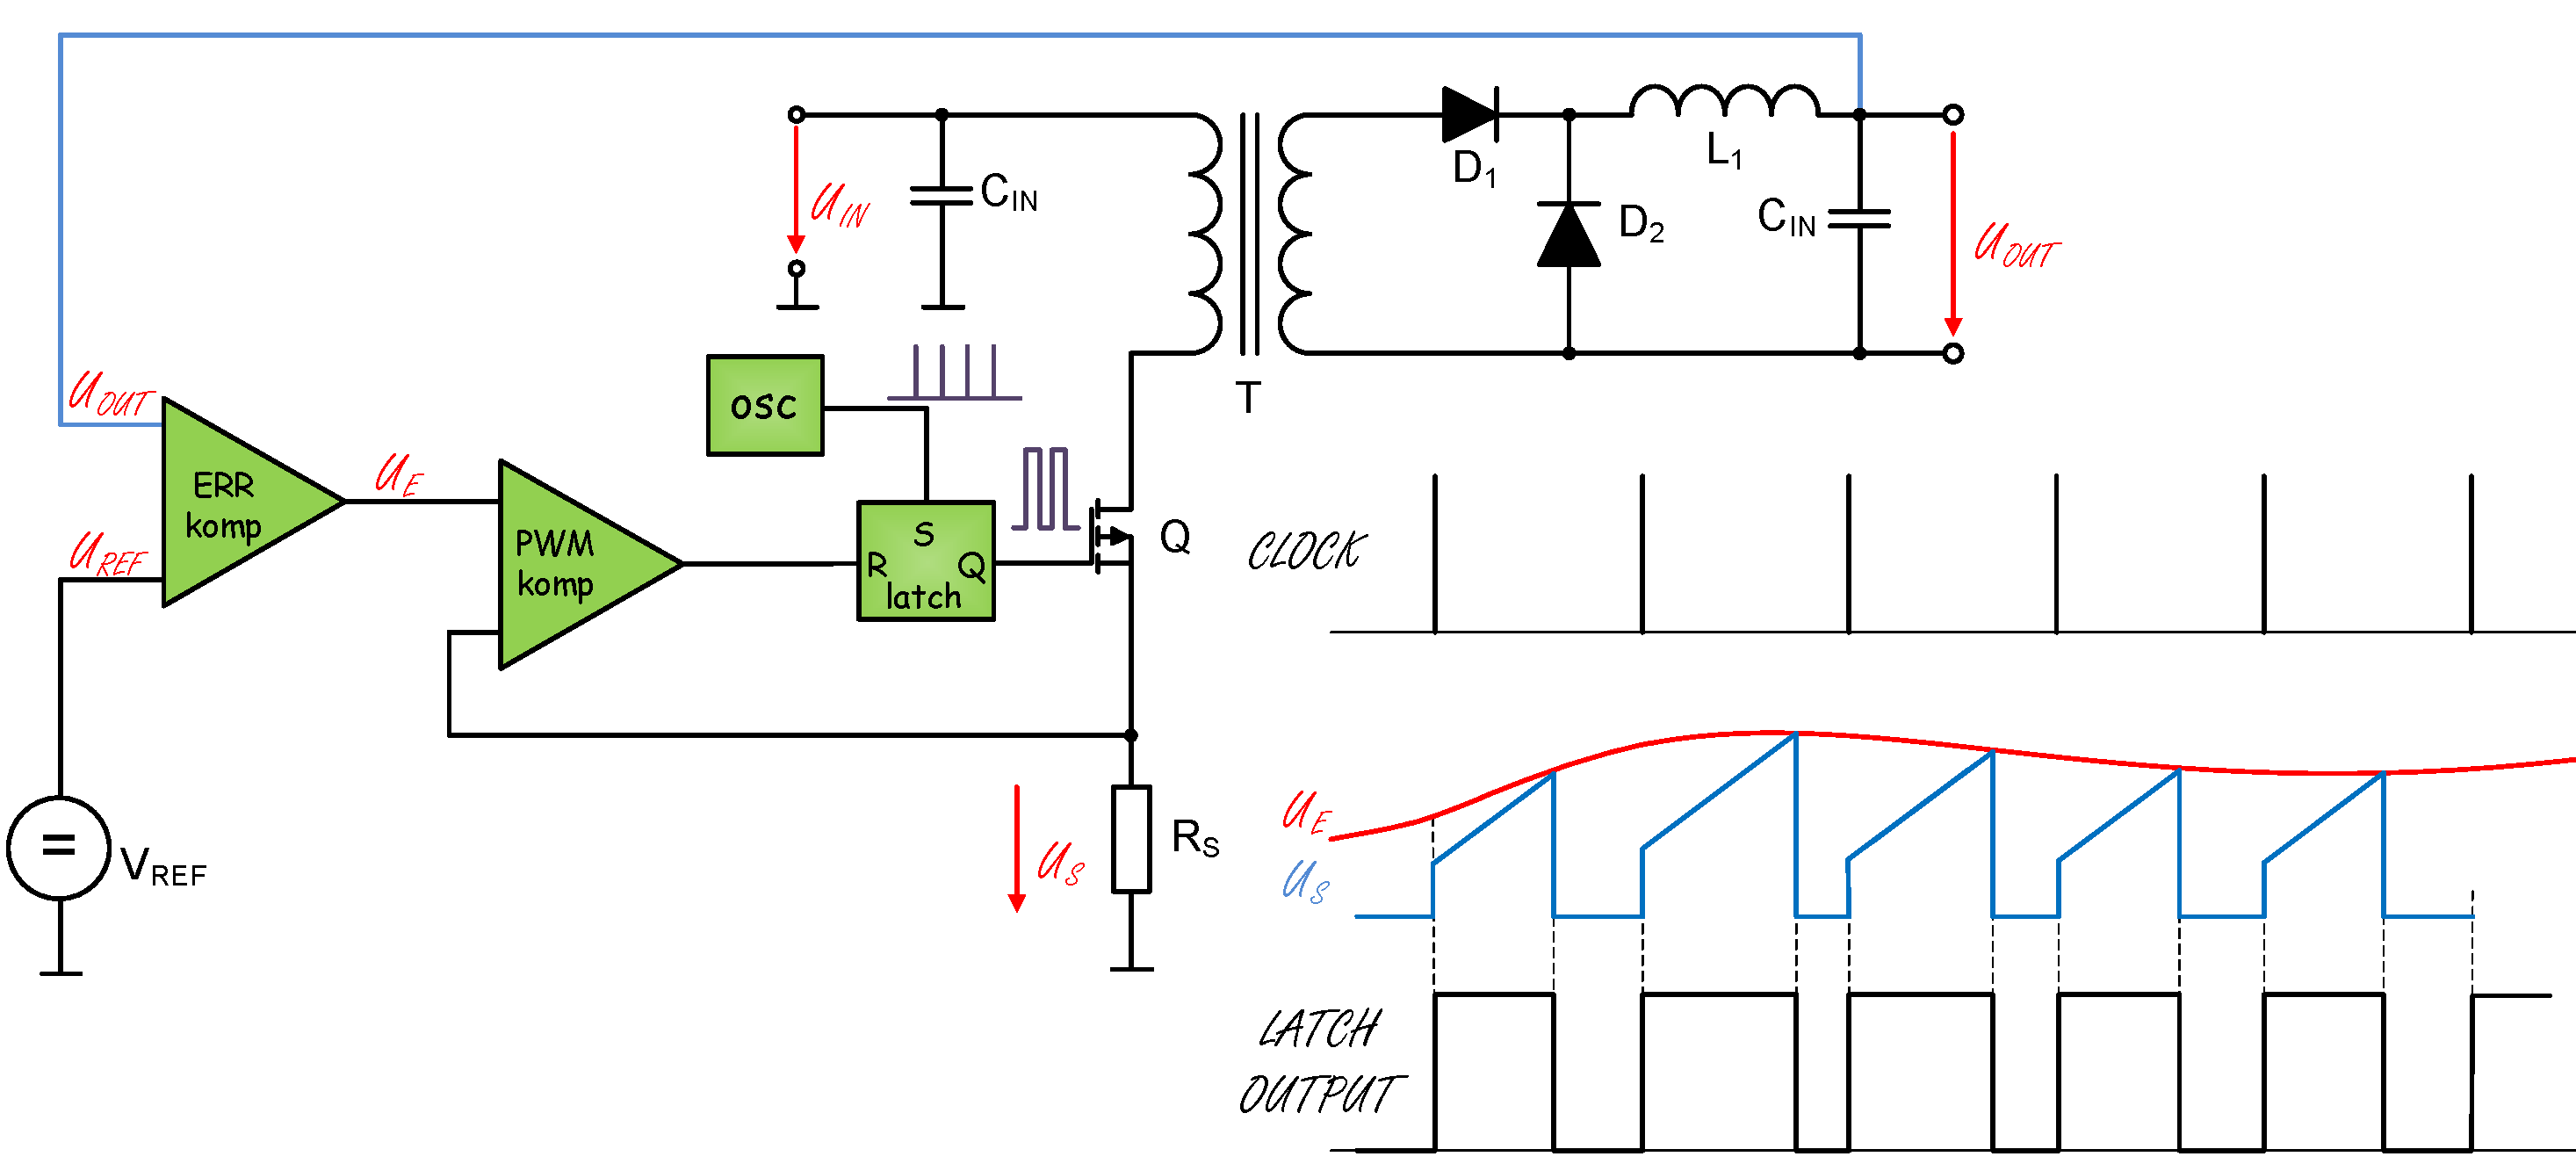
\includegraphics[width=0.9\linewidth]{unitrode_current_mode_control.pdf}
        \caption[Regulátor s proudovým řízením]{Regulátor s proudovým řízením - Current mode
                 control [\cite{SLUA119}]}
        \label{ENZ:fig_I_mode_cntrl}
      \end{figure}
  
      Výhody:
      \begin{itemize}[noitemsep]
        \item Input voltage feed-forward, resulting in good open-loop line regulation.
        \item Simplified loop --inductor pole and 2nd order characteristic eliminated.
        \item Optimum large-signal behavior.
        \item No conditional loop stability  problems.
        \item Flux balancing (symmetry correction) in push-pull circuits.
        \item Automatic pulse-by-pulse current limiting.
        \item Current sharing of paralleled supplies for modular power systems.
        \item Less complexity/cost (current sense/amp is not an added complication).
      \end{itemize}
  
      Nevýhody (continuous  mode  only):
      \begin{itemize}[noitemsep]
        \item Peak/avg. current error and instability --slope compensation
        \item Noise immunity is  worse because of  shallower ramp.
        \item Half Bridge runaway
        \item DC open loop load regulation is worse.
        \item (1-D) current error in Boost or Flyback circuits.
        \item Loop irregularities with multiple output buck circuits.
      \end{itemize}
  
    \subsection{Realizace zpětné vazby regulátorem TL431}
      Showing compensation circuits around an op amp is an interesting thing, but the industrial 
      design world differs in reality. The TL431 presence in feedback systems is overwhelming, and 
      few designs still use a true operational amplifier. Why? Because the TL431 already includes a 
      stable and precise reference voltage with an error amplifier. Even if its open-loop gain 
      cannot compete against a true op amp, it is good enough for the vast majority of product 
      definitions. 
      
      What exactly is a TL431? Figure 3.54 shows the internal arrangement of the device. You can 
      observe a reference voltage of 2.5 V biasing an operational amplifier inverting input. The 
      output drives a bipolar transistor, actually making the TL431 a shunt regulator: When the 
      voltage on the reference pin (R) is below 2.5 V, the transistor remains blocked open and the 
      TL431 is transparent to the circuit. As soon as the voltage exceeds the reference, the 
      transistor starts to conduct and a current circulates inside the device. If an optocoupler 
      LED appears in series with the cathode, it becomes possible to build an optoisolated feedback 
      system. Figure 3.55 shows how most of today’s power supplies implement a TL431: here, in a 
      typical flyback converter.
      \begin{figure}[ht!]
        \centering  
        \subcaptionbox{\label{enz:fig_tl431_01a}}{\luafigure[0.35]{TL431_01a.png}}
        \subcaptionbox{\label{enz:fig_tl431_01b}}{\luafigure[0.25]{TL431_01b.png}}
        \caption{The internal equivalent schematic of the TL431 featuring a 2.5V reference voltage  
          \cite[s.~43]{Basso2008}} 
        \label{enz:fig_tl431_01}
      \end{figure}
      
      The TL431 also exists in different precision versions, depending on what you are looking for. 
      In some cases in which you need output voltages below 2.5 V, the TLV431 might be a good 
      choice. The latter also features a smaller minimum biasing current compared to the TL431. 
      Regarding low standby current shunt regulators, it is worth mentioning the NCP431 that can 
      also operate down to 40 mA, but it accepts a maximum voltage up to 36 V. It can be a good 
      advantage in low-standby-power designs. The following array compares all versions.
  
      \begin{figure}[ht!]
        \centering
        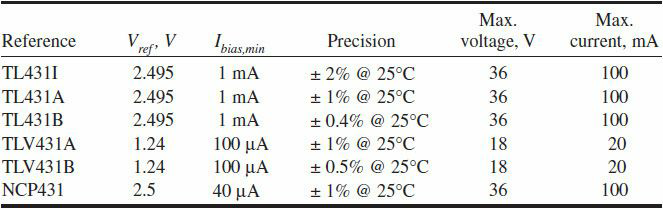
\includegraphics[width=0.7\linewidth]{TL431_03.png}
        \caption{Different versions of the TL431\cite[s.~43]{Basso2008}}
        \label{enz:fig_tl431_03}
      \end{figure}
      Appendix 3B describes the SPICE models of a behavioral TL431, which we extensively used in 
      all the book examples. This model can work on IsSpice or PSpice and has proved to properly 
      reflect reality.
      
      In Fig. 3.55, the resistive network Rupper-Rlower senses the output voltage and biases the 
      TL431 reference pin. When the output is above the reference, the TL431 reduces its cathode 
      voltage and increases the LED current. This, in turn, reduces the feedback set point, and the 
      converter delivers less power. On the contrary, when the output is below the target, the 
      TL431 almost leaves the cathode open and stops pumping current into the LED. As a result, the 
      primary feedback allows for more output power, pushing the converter to increase the output 
      voltage until the TL431 detects the target is reached. The converter can accept two different 
      optocoupler configurations, described as solutions A and B:
      
      \begin{figure}[ht!]
        \centering
        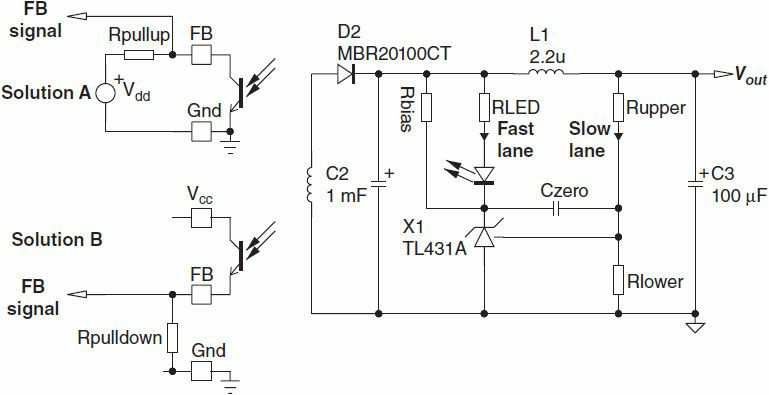
\includegraphics[width=0.8\linewidth]{TL431_02.png}
        \caption{A TL431 monitors a portion of the output voltage and activates an optocoupler LED 
                 to transmit the feedback information to the nonisolated primary side. 
                 \cite[s.~43]{Basso2008}}
        \label{enz:fig_tl431_02}
      \end{figure}
       
      \begin{itemize}[noitemsep]
        \item Solution A: This is a common emitter configuration as found on popular controllers 
              such as ON Semiconductor’s NCP1200 series. Bringing the FB pin down reduces the peak 
              current in this current-mode controller. This solution also exists on UC384X-based 
              designs where the collector can directly drive the output of the internal op amp.
        \item Solution B: In this common collector configuration, the emitter pulls high the FB pin 
              to reduce the duty ratio or the peak current set point. This option usually requires 
              an inverting amplifier inside the controller.
      \end{itemize}
    

  % -------------- Sbírka katalogových zapojení neizolo\-va\-ných měnič ů---------------------------
  \section{Sbírka katalogových zapojení neizolo\-va\-ných měničů}\label{aes:sec009}
    Existují dvě možnosti, jak provádět řízení pomocí PWM odlišující se \emph{typem zpětné
    vazby}, která je buď čistě \textbf{napěťovou vazbou} (\emph{voltage mode control}), nebo
    \emph{napěťovou vazbou s vnitřní proudovou smyčkou} (\emph{current mode control}). V
    následující diskusi se pokusíme konzistentním způsobem vysvětlit vlastnosti obou řídících
    algoritmů (slua119)
    
    \subsection{Zdroj symetrického napětí s jedním induktorem}
      \begin{figure}[ht!]
        \centering
        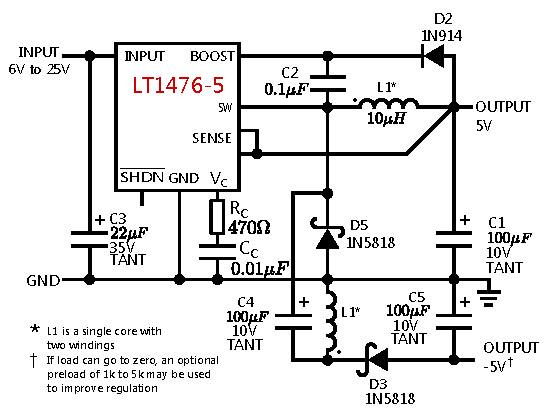
\includegraphics[width=0.8\linewidth]{LT1376_dual_output_reg.pdf}
        \caption[Spínaný zdroj napětí $\pm5 V$ vystačí s jedinou indukčností s dvojím
                 vinutím]{Spínaný zdroj napětí $\pm5 V$ vystačí s jedinou indukčností s dvojím
                 vinutím. \cite{DN100}. Linear Technology Corp. (Dual Output Regulator Uses Only
                 One Inductor)}
        \label{enz:fig_LT1376_cir1}
      \end{figure}
      Toto řešení na obr. \ref{enz:fig_LT1376_cir1} nabízí spínaný zdroj symetrického napětí za
      použití několika dalších součástek a induktoru s dvojím vinutím. Základní části zdroje je
      napěťový regulátor snižující vstupní kladné napětí založený na obvodu \emph{LT1376-5} se
      spínacím kmitočtem 500 kHz a možností zatížení proudem až 1,5 A.

      \begin{figure}[ht!]
        \centering
        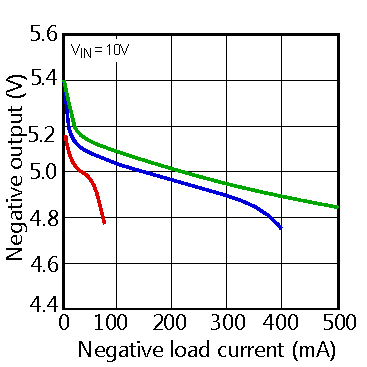
\includegraphics[width=0.4\linewidth]{LT1376_dual_output_reg_performance.pdf}
        \caption{Zatěžovací charakteristika záporné větve.}
        \label{enz:fig_LT1376_cir1_perform}
      \end{figure}

      Druhá polovina induktoru $L_1$ společně s $D_3$, $C_5$ a $C_4$ je určena pro tvorbu
      záporného napětí pomocí \textbf{SEPIC topologie} - \emph{Single Ended Primary Inductance
      Converter}. Kondenzátor $C_4$ vnucuje oběma vinutím stejné napětí. Bez něho pracuje tato
      část jako blokující měnič (\textbf{flyback}), která by sice poskytla -5V, ale jen naprázdno
      se značnou závislostí na zátěži (nedokonalá vazba mezi vinutími).

%---------------------------------------------------------------------------------------------------
